\documentclass{beamer}
\usetheme{metropolis}            % Clean academic theme
\usecolortheme{seahorse}        % Built-in theme

\setbeamertemplate{footline}[frame number]
\usepackage{graphicx}
\graphicspath{{images/}{images/scientists/}{images/emojis/}{images/camera/}}
\usepackage{overpic}
\usepackage{subcaption}
\usepackage{siunitx-v2}
\DeclareSIUnit{\siemens}{S}
\DeclareSIUnit{\faraday}{F}
\DeclareSIUnit{\electron}{e}
\DeclareSIUnit{\gauss}{G}
\DeclareSIUnit{\ppm}{ppm}
\usepackage{mhchem}
\usepackage{physics}
\usepackage{caption}
\captionsetup[figure]{labelformat=empty}
\usepackage[rightcaption]{sidecap}
\usepackage{booktabs}
\usepackage{wrapfig}
\usepackage{xcolor}
\definecolor{VignanBlue}{RGB}{0,102,204}   % Strong blue
\definecolor{VignanRed}{RGB}{200,30,60}    % Crimson red (optional for highlights)
%
\newtheorem{derivation}{Derivation}
\setbeamercolor{guesstimate}{fg=blue,bg=blue!10}
%
\setbeamerfont{theorem body}{series=\normalfont}
%
\newenvironment{learningobjectives}[1][]{%
	\begin{block}{Learning Objectives \hfill
		\raisebox{0ex}{
\includegraphics[height=2ex]{target}}
		} }{\end{block}
}
%
\newenvironment{question}[1][]{%
	\begin{block}{Question \hfill
			\raisebox{0ex}{
\includegraphics[height=2ex]{question}}
		}\small}{\end{block}
}
%
\newenvironment{guesstimate}[1]{%
	\begin{block}{Estimate: {#1} \hfill
			\raisebox{0ex}{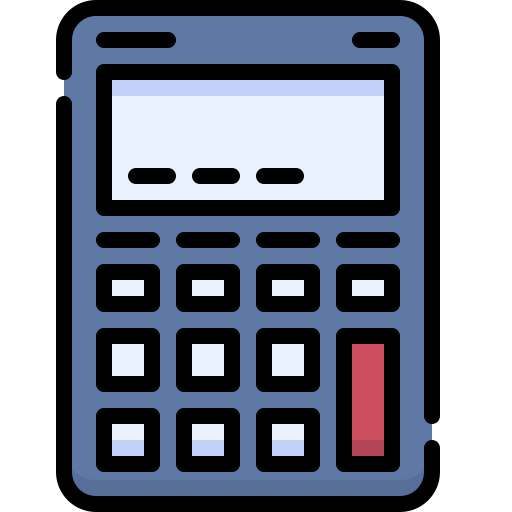
\includegraphics[height=2ex]{calculator}}
		} \small}{\end{block}
}
%
\newenvironment{keyinsight}[1][]{%
	\begin{block}{\centering Key Insight \hfill
		\raisebox{0ex}{
\includegraphics[height=2ex]{light_bulb}}
		}}{\end{block}
	}
\newenvironment{trends}[1][]{%
	\begin{block}{Trends \hfill
			\raisebox{0ex}{
\includegraphics[height=2ex]{trend}}
		} \small\centering}{\end{block}
}
\newenvironment{disclaimer}[1][]{%
	\begin{block}{Disclaimer \hfill
			\raisebox{0ex}{
\includegraphics[height=2ex]{disclaimer}}
	}}{\end{block}
}
\newif\ifshowhidden
\showhiddenfalse
%
\title[Engineering Physics]{Engineering Physics (2025) \\ Course code
	25PY101-S2 \\ Module 1 Unit 1: Classical Free Electron Theory}
\author{Course Instructor:\\ 
	{\color{VignanBlue} Dr. Sreekar Guddeti}\\
	Assistant Professor in Physics\\
	Department of Science and Humanities \\
	{\color{VignanRed}Vignan's Foundation for Science, Technology and Research}
}
%
\begin{document}
	\frame{\titlepage}
	%\begin{frame}[label=syllabus]{Course Structure and Outline}
%
	\begin{enumerate}
		\item Number of credits	\hfill 4
		\item Number of hours per week \hfill 8
		\item Decomposition of hours \hfill L(3), T(0), P(2), SL(3) 
		\item Number of Modules	\hfill 2
		\item Number of weeks per Module \hfill M1 (6), M2 (9)
	\end{enumerate}
	%
	\begin{table}
		\begin{tabular}{l l l}
			\toprule
			Module	&	Unit	&	Topic	\\
			\midrule
			Module 1	&	Unit 1	&	Classical Free Electron Theory \\
			&	Unit 2 	&	Quantum Mechanics	\\
			Module 2	&	Unit 1	&	Quantum Free Electron Theory	\\
			&	Unit 2	& 	Optoelectronics	\\
			&	Unit 3	&	Laser	\\
			\bottomrule
		\end{tabular}
		\caption{Course Outline.}
	\end{table}
\end{frame}	
%
\begin{frame}{Course Lectures: Module 1}
	%
	
	{
		\small	
		\begin{table}
			\begin{tabular}{ll}
				\toprule
				\multicolumn{2}{l}{Module 1}	\\
				\midrule
				Unit 1 	& Introduction to metals, expression for electrical conductivity \\
				& Introduction to semiconductors--intrinsic and extrinsic \\
				& Elec. conductivity of s.c. -- intrinsic and extrinsic (Quantitatively) \\
				& Hall effect- applications, Concept of Panchabhuta -- five elements	\\
				Unit 2 & Introduction to Quantum Mechanics, Dual nature of radiation \\
				& de Broglie’s concept of matter waves, Uncertainty principle \\
				& Schrödinger’s time-independent wave equation\\ & Particle confined in a one-dimensional infinite potential well\\
				& Quantum dots \\ 
				& Finite potential well- Quantum Tunneling \\
				& Scanning tunneling microscope, tunneling diode (Qualitative)	\\
				&	Kanada's atomic theory (paramanu)	\\
				\bottomrule
			\end{tabular}
			\caption{Topics of Module 1.}
		\end{table}
	}
\end{frame}
%
%
\begin{frame}{Course Lectures: Module 2}
	%
	
	{
		\tiny
		
		\begin{table}
			\begin{tabular}{ll}
				\toprule
				\multicolumn{2}{l}{Module 2}	\\
				\midrule
				Unit 1 & Quantum free electron theory, Fermi-Dirac distribution\\
				& Electronic specific heat of solids, Density of states (qualitative) \\
				& Success and Failures of quantum free electron theory of solids \\
				& E-k diagram- classification of materials based on bands in solids \\
				& Fermi level in semiconductors -- intrinsic and extrinsic. \\
				%
				Unit 2 & p-n junction diode- forward and reverse bias conditions \\
				& Solar cell-construction, working-characteristics, applications \\
				& Direct and indirect bandgap semiconductors \\
				& LED-construction, working characteristics,  applications.	\\
				& Photodiode, construction, working characteristics, applications \\
				Unit 3 & Introduction to lasers \\
				& Normal light vs. laser light -- characteristics of laser light \\
				& Stimulated absorption, Spontaneous and Stimulated emission \\
				& population inversion, pumping \\
				& Optical resonator-lasing mechanism	\\
				& Diode laser -- construction,working and applications \\
				& Optical fibre -- Total internal reflection, acceptance angle, \\
				& numerical aperture, communications	\\
				\bottomrule
			\end{tabular}
			\caption{Topics of Module 2.}
		\end{table}
	}
\end{frame}
%
\begin{frame}{Course Self-Learning}
	%
	\vspace{-0.5em}
	{
		\footnotesize
\begin{itemize}
	\item At-least \textbf{three hours per week} of self-learning.
		%
	\item	Textbooks
		\begin{enumerate}
			\item M. N. Avadhanulu, “Engineering Physics”, S. Chand publications 2010.
			\item Donald A. Neamen, “Semiconductor Physics and Devices: Basic principle”, 4th edition, McGraw-Hill, New York, 2012.
			%
		\end{enumerate}
		%
	\item References
		%
		\begin{enumerate}
			\item D. Halliday, R. Resnick and J. Walker, “Fundamentals of Physics”, 6th edition, John Wiley and Sons, New York, 2001.
			\item M. N. Avadhanulu, “Engineering Physics”, S. Chand publications 2010.
			\item Charles Kittel, “Introduction to solid state physics”, 7th edition , Wiley, Delhi, 2007.
			\item David J. Griffiths, “Introduction to Electrodynamics”, 3rd edition, Prentice Hall of India, New Delhi, 2012.
			\item Ashcroft and Mermin, “Solid State Physics”, International student edition, 2008.
			%
		\end{enumerate}
\end{itemize}
	}
\end{frame}
%
\begin{frame}{Course Practices -- Module 1}
	\begin{enumerate}
		\item \textcolor{green}{Determination of Energy Band gap of p-n junction diode}.
		\item \textcolor{green}{Hall effect -- Determination of Hall effect}.
		\item \textcolor{green}{Photoelectric effect -- Determination of Planck's constant}.
		\item \textcolor{red}{Seebeck effect -- To study the variation of thermoemf of a copper-constantan thermocouple with temperature}.
		\item \textcolor{green}{Thermistor -- To study the characteristics of Thermistor and to find its type}.
	\end{enumerate}
\end{frame}
\begin{frame}{Course Practices -- Module 2}
	\begin{enumerate}
		\item \textcolor{red}{Study the characteristics of diode}.
		\item \textcolor{green}{Determination of efficiency and Fill factor of a solar cell}.
		\item \textcolor{red}{Determine the efficiency and fill factor of solar cells in Parallel and series combinations}.
		\item \textcolor{green}{Study the \(I-V\) characteristics of LED}.
		\item \textcolor{green}{Optical fibre – Determination of Numerical aperture – Acceptance angle}.
		\item \textcolor{red}{Determination of attenuation in Optical fiber}.
		\item \textcolor{green}{Laser - Determination of wavelength}.
		\item \textcolor{red}{Determination of the slit width from Fraunhofer diffraction pattern using LASER beam}.
		\item \textcolor{red}{Demonstration of monochromatic nature of laser light comparing with ordinary light by the principle of dispersion by using Prism}.
		%
	\end{enumerate}
\end{frame}
%
%
\begin{frame}{Course Outcomes (COs)}
	\begin{enumerate}
		\item Comprehend the characteristics of metals and semiconductors based on electrical properties.
		\item Apply the principles of quantum mechanics to unravel the latest technical developments such as quantum dots and scanning tunneling microscope.
		\item Categorize the solids based on band theory.
		\item  Evaluate p-n junction diodes in optoelectronic devices such as solar cells, LED’s and photodiodes.
		\item Apply the fundamental principles of Lasers and optical finer systems to explain lasing action in semiconducting laser diode laser and light propagation in optical fibers for communication.
		\item Exhibit scientific communication skills by preparing structured laboratory reports, presenting experimental findings, and following standard documentation practices.
	\end{enumerate}
	%
\end{frame}
%
\begin{frame}{Program Outcomes (POs)}
	%
	\begin{table}
		\centering
		\begin{tabular}{ll}
			\toprule
			PO code	&	PO title	\\
			\midrule
			PO1	& 	Engineering Knowledge	\\
			PO2	&	Problem Analysis	\\
			PO3	&	Design/Development of Solutions	\\
			PO4	&	Conduct investigations of Complex problems	\\
			PO5	&	Engineering Tool Usage	\\
			PO6	&	The Engineer and the World	\\
			PO7	&	Ethics	\\
			PO8	&	Individual and Collaborative Team work	\\
			PO9	&	Communication	\\
			P10	&	Project Management and Finance	\\
			P11	&	Life-long learning	\\
			\bottomrule
		\end{tabular}
		\caption{Program outcomes.}
	\end{table}
\end{frame}
\begin{frame}{Mapping of COs to POs}
	\begin{table}
		\begin{tabular}{llll}
			\toprule
			CO 	&	BT	&	Module	&	Mapping with PO (Level)	\\
			\midrule
			1 	&	Understand	&	1	&	1(3), 2(3), 3(2),4(2), 9(3),10(3),11(2) \\
			2	& 	Apply	&	1	&	1(3), 2(3), 3(3), 4(2), 9(3),10 (3) \\
			3	& 	Analyze	&	2	&	1(3), 2(3), 3(3), 4(2), 11(2)	\\
			4	& Evaluate	&	2	&	1(3), 2(3), 3(3), 4(2), 9(3),10 (3),11(2)	 \\
			5	&	Apply	&	2	&	1(3), 2(3), 3(3), 4(2),5 (2), 9(3),10 (3),11(2) \\
			6	&	Create	&	2	&	2(2), 4(3),  9(2),  10(3), 11(1) \\
			%
			\bottomrule
		\end{tabular}
		\caption{CO-to-PO mapping.}
	\end{table}
	%
	\begin{block}{Sustainable development goals}
		\begin{figure}
			
\includegraphics[width=0.8\textwidth]{sustainable_development_goals}
		\end{figure}
	\end{block}
\end{frame}
%
	%
	\begin{frame}{M1U1 Plan}
	%
	\tableofcontents
	%
\end{frame}
%
%
\begin{frame}<0>[label=plan]{M1U1 Plan}
	%
	\tableofcontents[currentsection]
	%
\end{frame}
	%
	\section{Condensed matter}
	%
	%\ifshowhidden
	%
\againframe{plan}
%
\begin{frame}{Lecture plan}
	\begin{learningobjectives}
		\begin{itemize}
			\item Condensed matter at macroscopic scale
			\item Classification of condensed matter based on conductivity
			\item Nature of metals
			\item Classical electron theory of metals -- Assumptions
			\item Ohm's law for metals -- Conductivity
			\item Application of metallic conductivity
		\end{itemize}
	\end{learningobjectives}
\end{frame}
\begin{frame}{Discovery of material}
	\begin{figure}
		\centering
		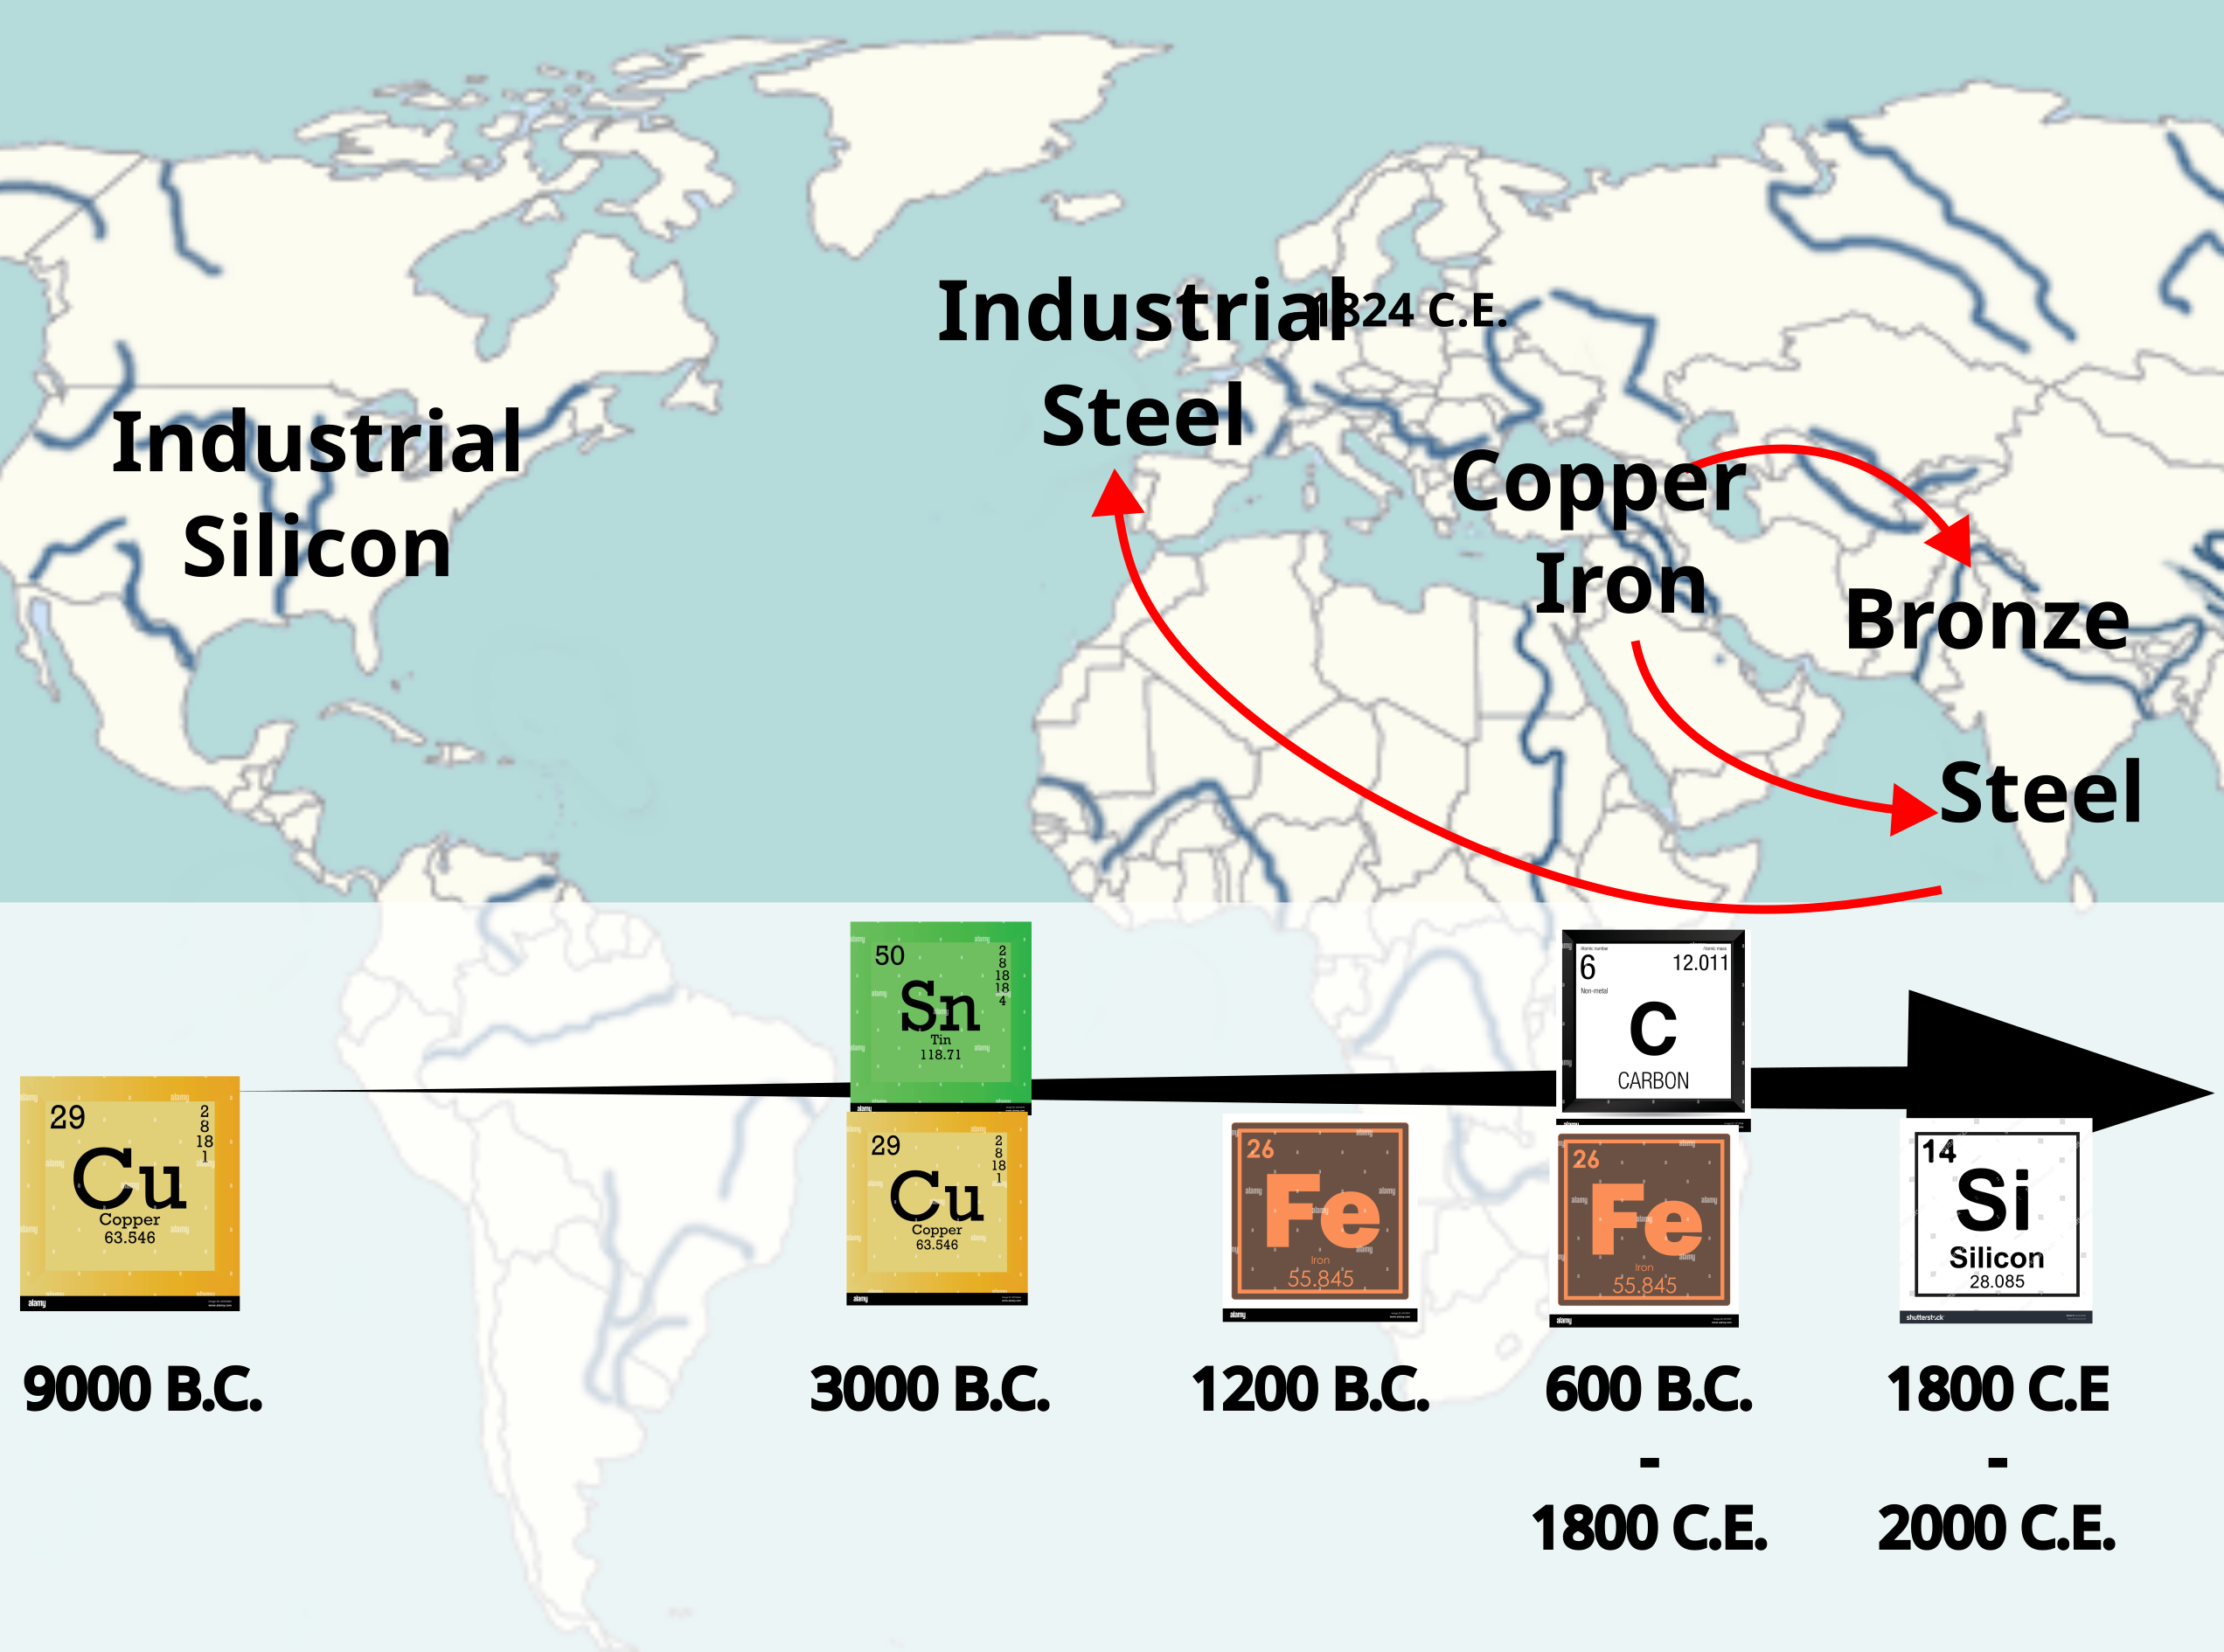
\includegraphics[height=0.6\textheight]{ages_human_civilization_spacetimeline}
		\caption{Civilization spacetimeline: Copper \(\rightarrow\) Bronze \(\rightarrow\) Iron \(\rightarrow\) Steel \(\rightarrow\) Silicon}
	\end{figure}
	%
	\begin{keyinsight}
		Material defines the age.
	\end{keyinsight}
\end{frame}
%
\begin{frame}{Condensed matter}
	\begin{itemize}
		\item Material in the liquid or solid form is called \textbf{condensed matter}.
		\item Condensed matter is further sub-classified based on  electrical, optical, magnetic, thermal, mechanical properties at the \textbf{macroscopic} scale.  In the case of electrical property, we apply electric field and classify the materials based on their conductivity.
		\item The macroscopic behaviour is related to the \textbf{microscopic} behaviour of electrons under applied ``forces''.
	\end{itemize}
	\begin{learningobjectives}
		To relate the macroscopic properties with the microscopic behaviour of electrons in condensed matter.
	\end{learningobjectives}
\end{frame}
%
\begin{frame}{Classification of Condensed Matter by Conductivity}
	%
	\begin{figure}
		\centering
		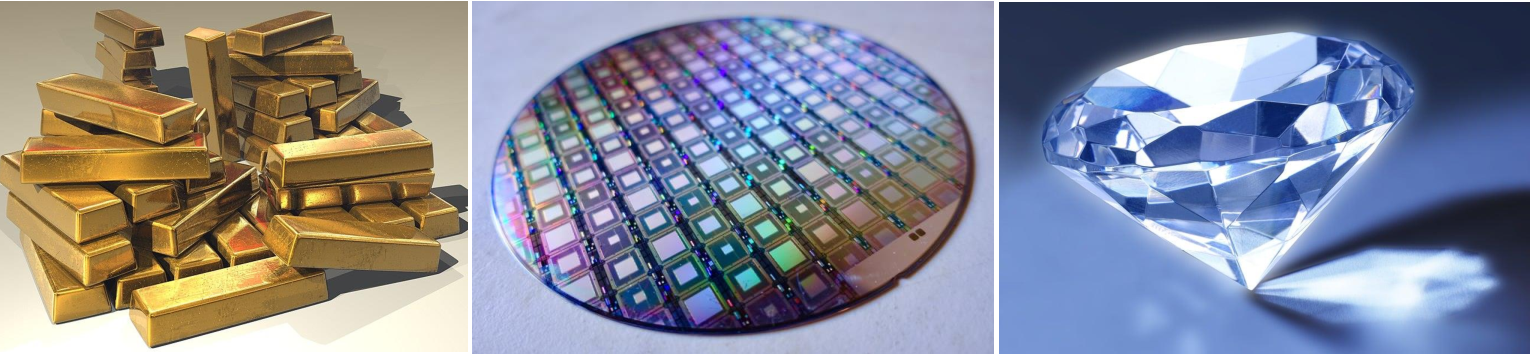
\includegraphics[width=\textwidth]{condensed_matter_electrical_classification}
		\caption{(a) Gold, a metal, (b) Silicon, a semiconductor, (c) Diamond, an insulator}
	\end{figure}
	%
	\begin{minipage}{0.85\textwidth}
		\begin{itemize}
			\item Conductivity is the measure of how easily electrons move under applied electric field. Its unit is \si{\per\ohm\per\metre} or \si{\siemens\per\metre} (S for Siemens).
			%
			\item Materials can be classified based on conductivity as:
			\begin{enumerate}
				\item \textbf{Metals}: High ($\sigma \sim 10^7$ S/m).
				\item \textbf{Semiconductors}: Intermediate ($\sigma \sim 10^{-4}$ S/m).
				\item \textbf{Insulators}: Negligible ($\sigma \sim 10^{-10}$ S/m).
			\end{enumerate}
		\end{itemize}
	\end{minipage}
	%
	\begin{minipage}{0.13\textwidth}
		\begin{figure}
			\centering
			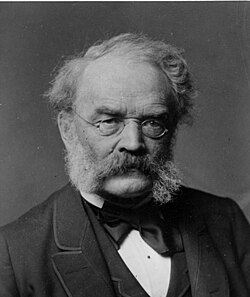
\includegraphics[width=\textwidth]{Werner_Siemens_1816-1892}
			\caption{\centering \footnotesize W. Siemens [1816-1892]}
		\end{figure}
	\end{minipage}
	
\end{frame}
%
\begin{frame}{Elemental phases}
	\begin{itemize}
		\item The electrical state of condensed matter is also called a \textbf{phase} -- similar to solid phase, liquid phase, etc.
	\end{itemize}
	\begin{figure}
		\centering
		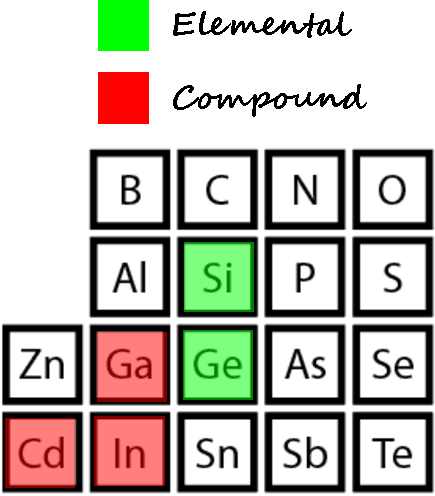
\includegraphics[height=0.5\textheight]{condensed_matter_periodic_table}
	\end{figure}
	%
	\begin{keyinsight}
		Most elemental phases are metals.
	\end{keyinsight}
\end{frame}
%
%
\begin{frame}{Conductivity of phases}
	%
	\begin{itemize}
		\item Conductivity \(\sigma\) is inversely related to resistivity \(\rho\) by \(\rho = \tfrac{1}{\sigma}\)
	\end{itemize}	
	%
	\begin{minipage}{0.75\textwidth}
		\begin{figure}
			\centering
			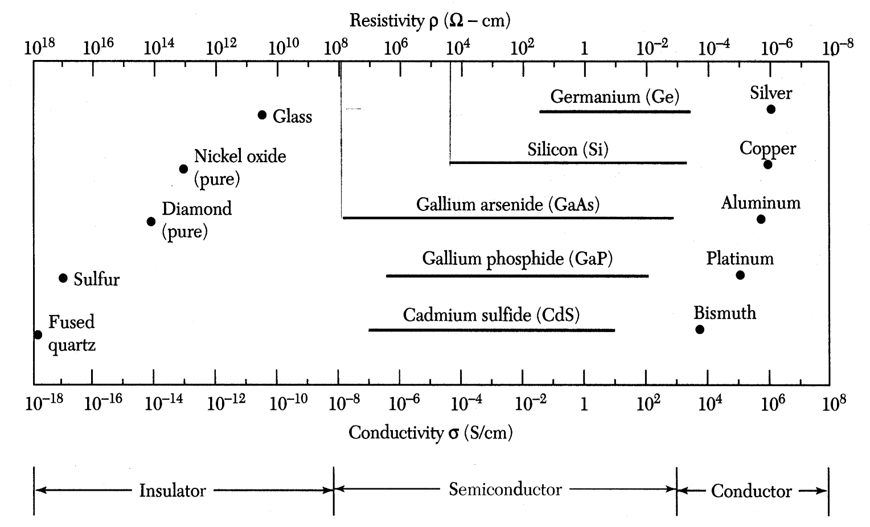
\includegraphics[width=\textwidth]{metals_resistivity_chart}
			%	\caption{Resistivity chart for metals, semiconductor and insulators}
		\end{figure}
	\end{minipage}
	%
	\hfill
	%
	\begin{minipage}{0.23\textwidth}
		{
			\footnotesize	
			\begin{table}
				\centering
				\begin{tabular}{l l }
					\toprule
					&		\(\rho\)	\\
					&		\si{\ohm\metre} \\
					\midrule
					\ce{Cu}	 &	\num{e-7}	\\
					\ce{Si} 	&	\num{e4}	\\
					\ce{SiO2}&	\num{e10}	\\
					\bottomrule
				\end{tabular}
			\end{table}
		}
	\end{minipage}
	%
	\begin{keyinsight}
		Conductivity spans ``orders of magnitude'' across phases.
	\end{keyinsight}
	%
\end{frame}
%
\begin{frame}{Early experiments:Avogadro number and Electron charge}
		\begin{figure}
		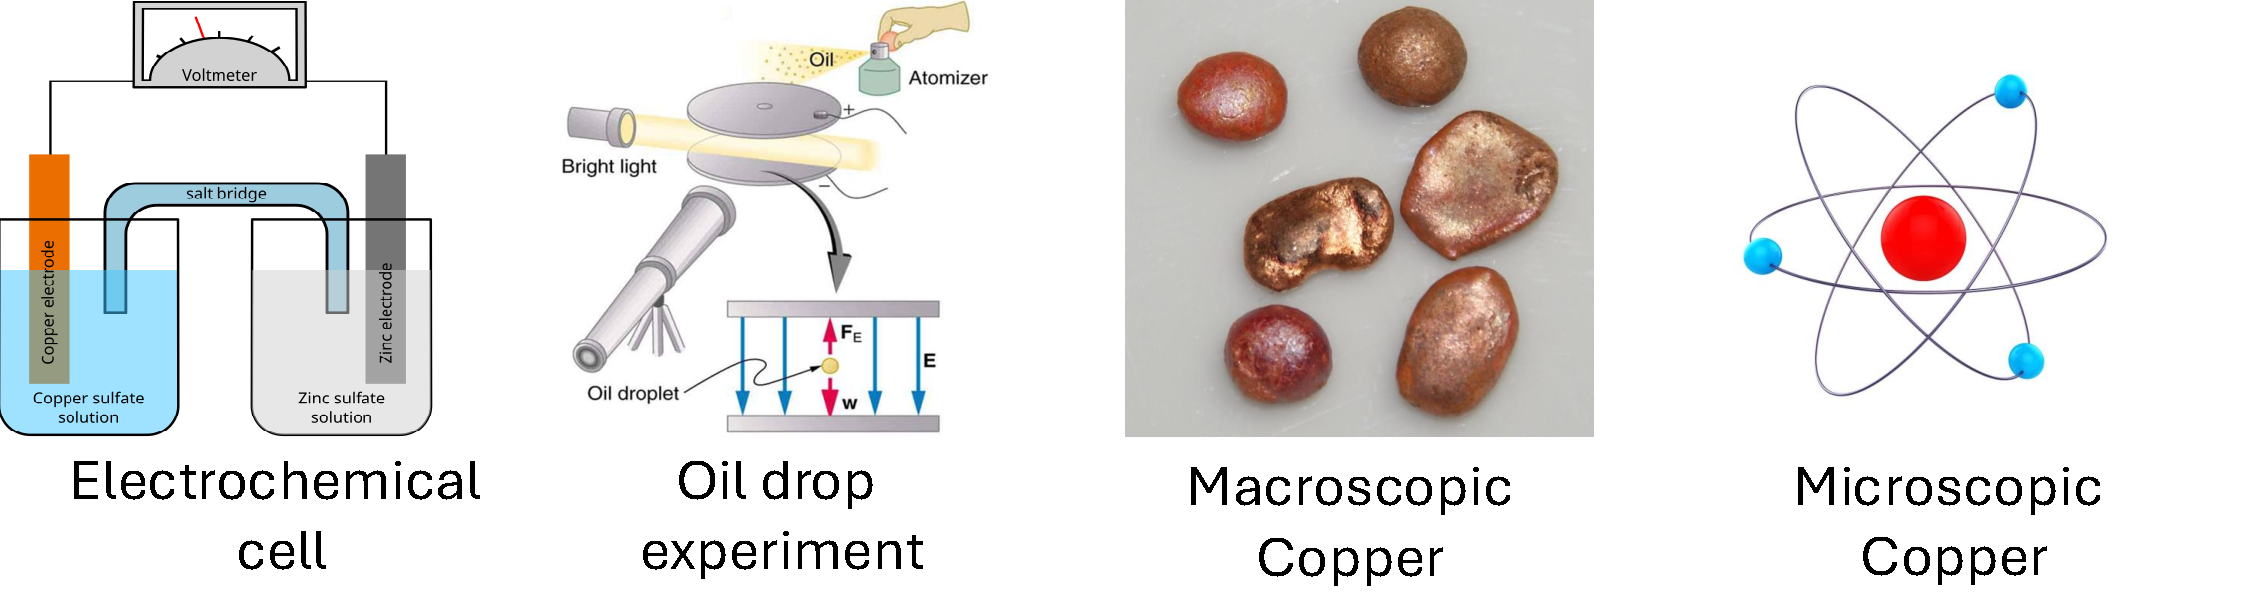
\includegraphics[width=2.2\textwidth]{condensed_macroscopic_to_microscopic}
	\end{figure}
	%
\end{frame}
%
\begin{frame}{Macroscopic \(\rightarrow\) microscopic}
	%
	\begin{figure}
		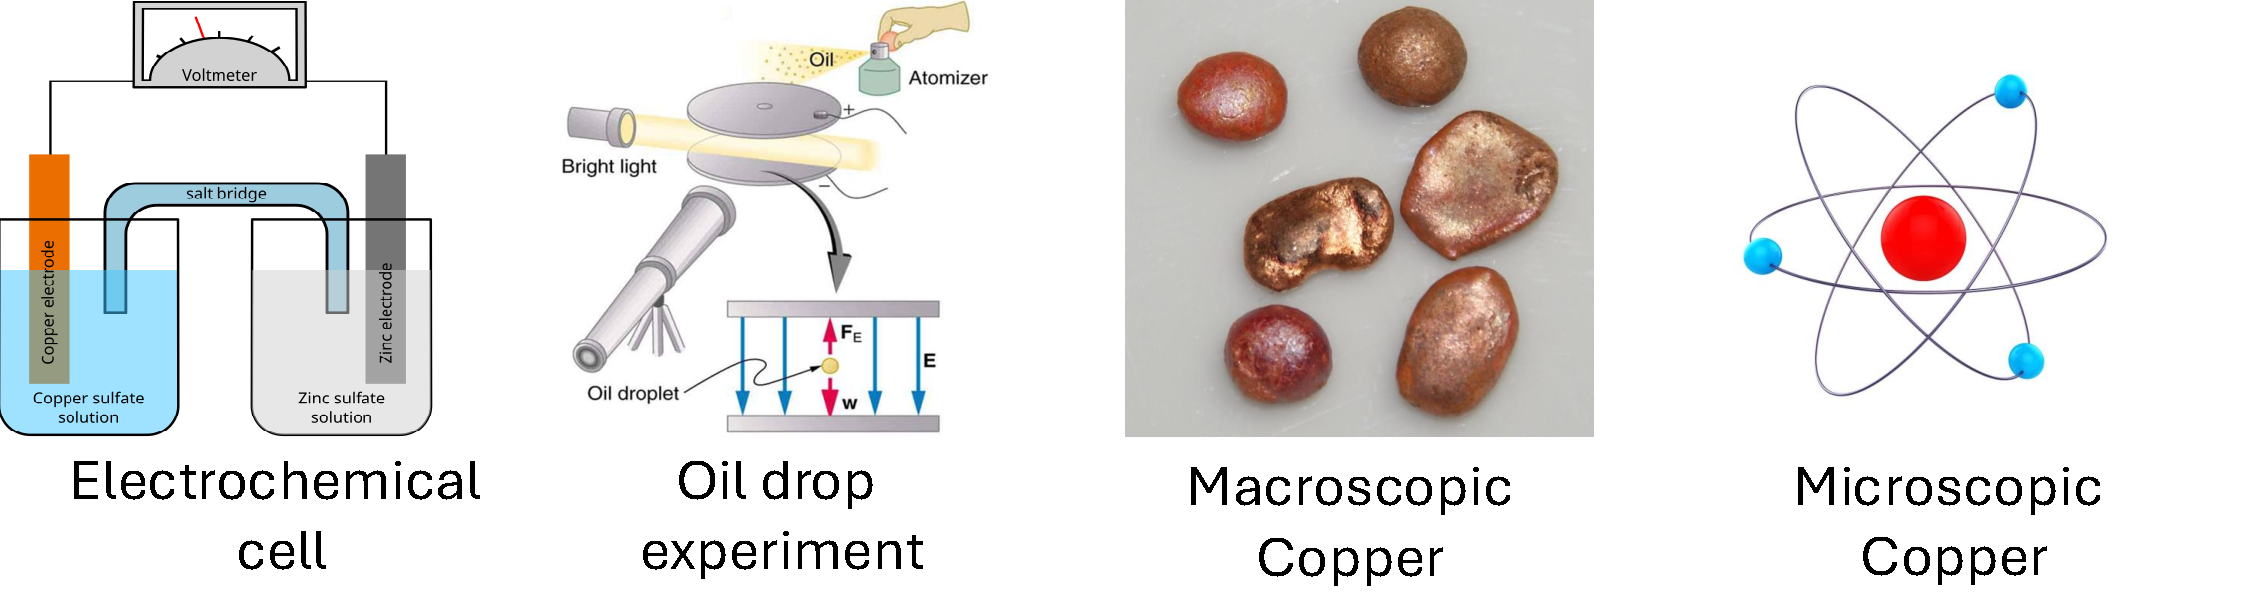
\includegraphics[width=\textwidth]{condensed_macroscopic_to_microscopic}
	\end{figure}
	%
	\begin{columns}
		\begin{column}[t]{0.7\textwidth}
			%
			\begin{guesstimate}{Avogadro number \(N_A\)}
				To electroplate \SI{63.5}{\gram} of copper, it takes \SI{2}{\faraday} of charge. [Hint: 1F (F for Faraday)= \SI{96,485}{\coulomb}, charge of electron \(e\) = \SI{1.602e-19}{\coulomb}]
			\end{guesstimate}
			%
			\begin{guesstimate}{Radius of atom}
				The density of copper is \SI{8.96}{\gram\per\centi\metre\cubed}.
			\end{guesstimate}
		\end{column}
		%
		\begin{column}[t]{0.28\textwidth}
			%
			\begin{figure}
				% Base image
				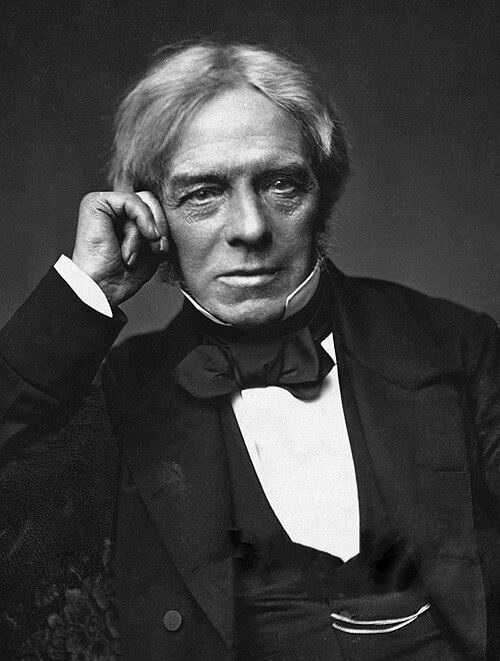
\includegraphics[width=0.48\textwidth]{Michael_Faraday_1791_1867}
				\begin{overpic}[width=0.48\textwidth]{Robert_Millikan_1868_1953}
					% Overlay image on top
					\put(0,0){\includegraphics[width=0.2\textwidth]{Alfred_Nobel_1833_1896}}
				\end{overpic}
				\caption{Faraday, Millikan}
			\end{figure}
		\end{column}
	\end{columns}
\end{frame}
%

	%\fi
	%
	\section{Metals}
	%
	%\ifshowhidden
	%
\againframe{plan}
%
\begin{frame}{Lecture Plan}
	\begin{learningobjectives}
		Learn the concept of 
		\begin{itemize}
			\item electrical conductivity,
			\item mobility, and
			\item relaxation time
		\end{itemize}
	\end{learningobjectives}
\end{frame}
%
\begin{frame}{Nature of Metal}
	%
	\begin{figure}
		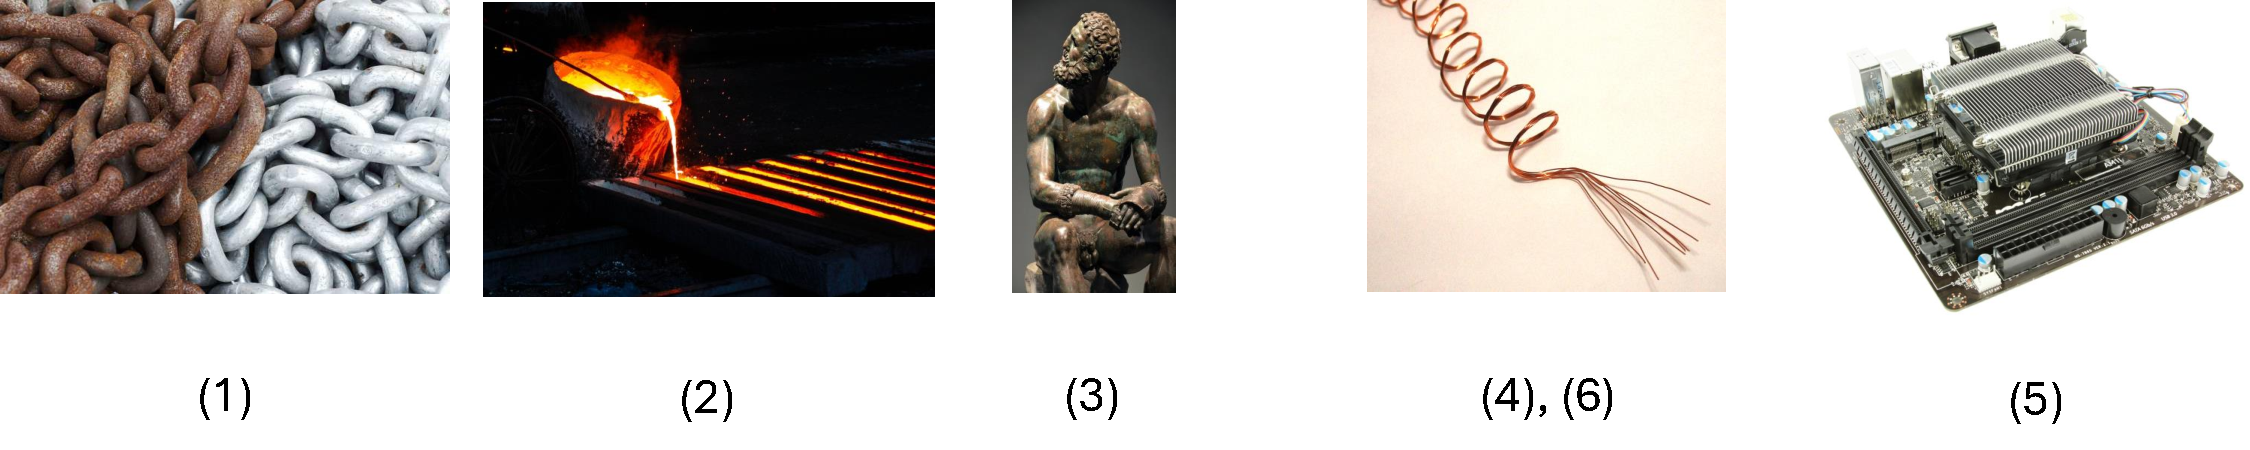
\includegraphics[width=\textwidth]{metals_nature}
	\end{figure}
	%
\begin{columns}
	\begin{column}[t]{0.6\textwidth}
		\begin{enumerate}
			\item Lustre (Shine)
			\item Solid with high \SI{~1000}{\celsius} melting points
			\item Malleable (capable of being shaped)
			\item Good electrical conductor
			\item Good thermal conductor
			\item Ductile (easy to draw wires)
		\end{enumerate}
	\end{column}
	%
	\begin{column}[t]{0.38\textwidth}
		\begin{block}{Chemistry}
			\begin{itemize}
				\item Metallic bonding
				\item Screening
			\end{itemize}
			%
			\begin{figure}
				\centering
				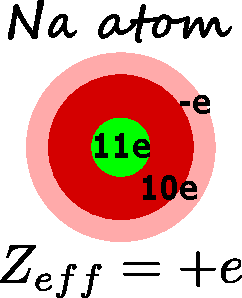
\includegraphics[width=0.4\textwidth]{metals_screening}
			\end{figure}
		\end{block}
	\end{column}
\end{columns}
	% 

\end{frame}
%
\begin{frame}{Metallic bonding \(\leftrightarrow\) electron gas}
	%
		\begin{figure}
			\centering
			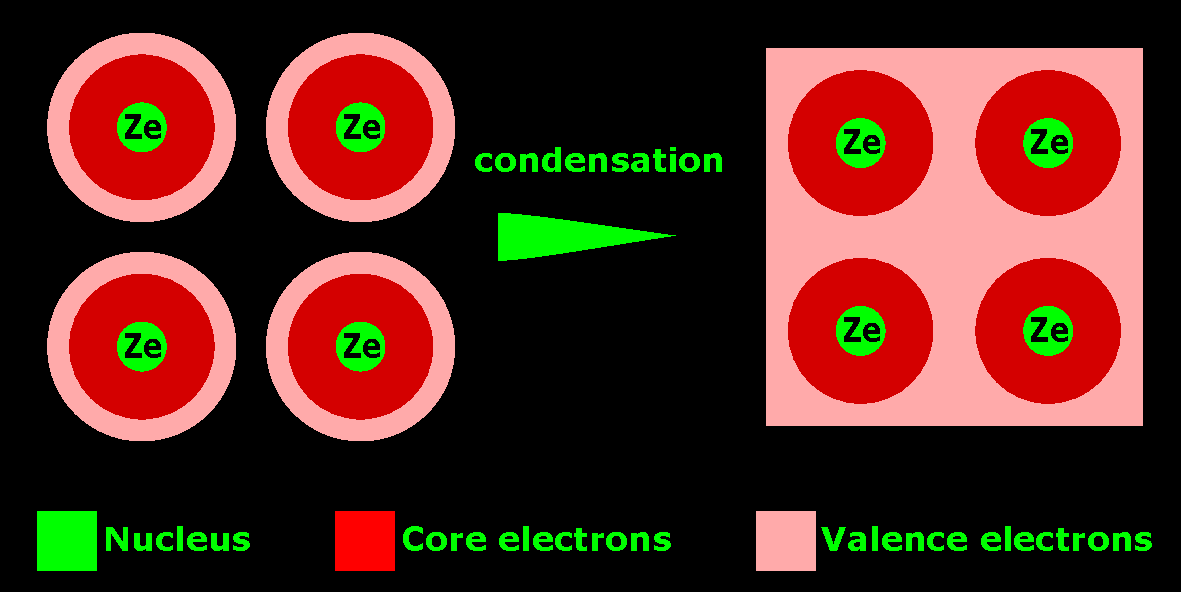
\includegraphics[width=0.9\textwidth]{metals_free_electron_gas}
			\caption{Valence electrons to electron ``gas''}
		\end{figure}
	%
		\begin{keyinsight}
		The properties of electron ``gas'' determines the nature of metal.
	\end{keyinsight}
	%
\end{frame}
%
\begin{frame}{Electron theories of metals}
\begin{columns}
	\begin{column}{0.3\textwidth}
		\begin{enumerate}
			\item Classical free electron theory
			\item Quantum free electron theory \hfill [M2 U3]
			\item Quantum band theory \hfill [M2 U3]
		\end{enumerate}
	%
	\end{column}
	%
	\begin{column}{0.68\textwidth}
			\begin{figure}
			\centering
			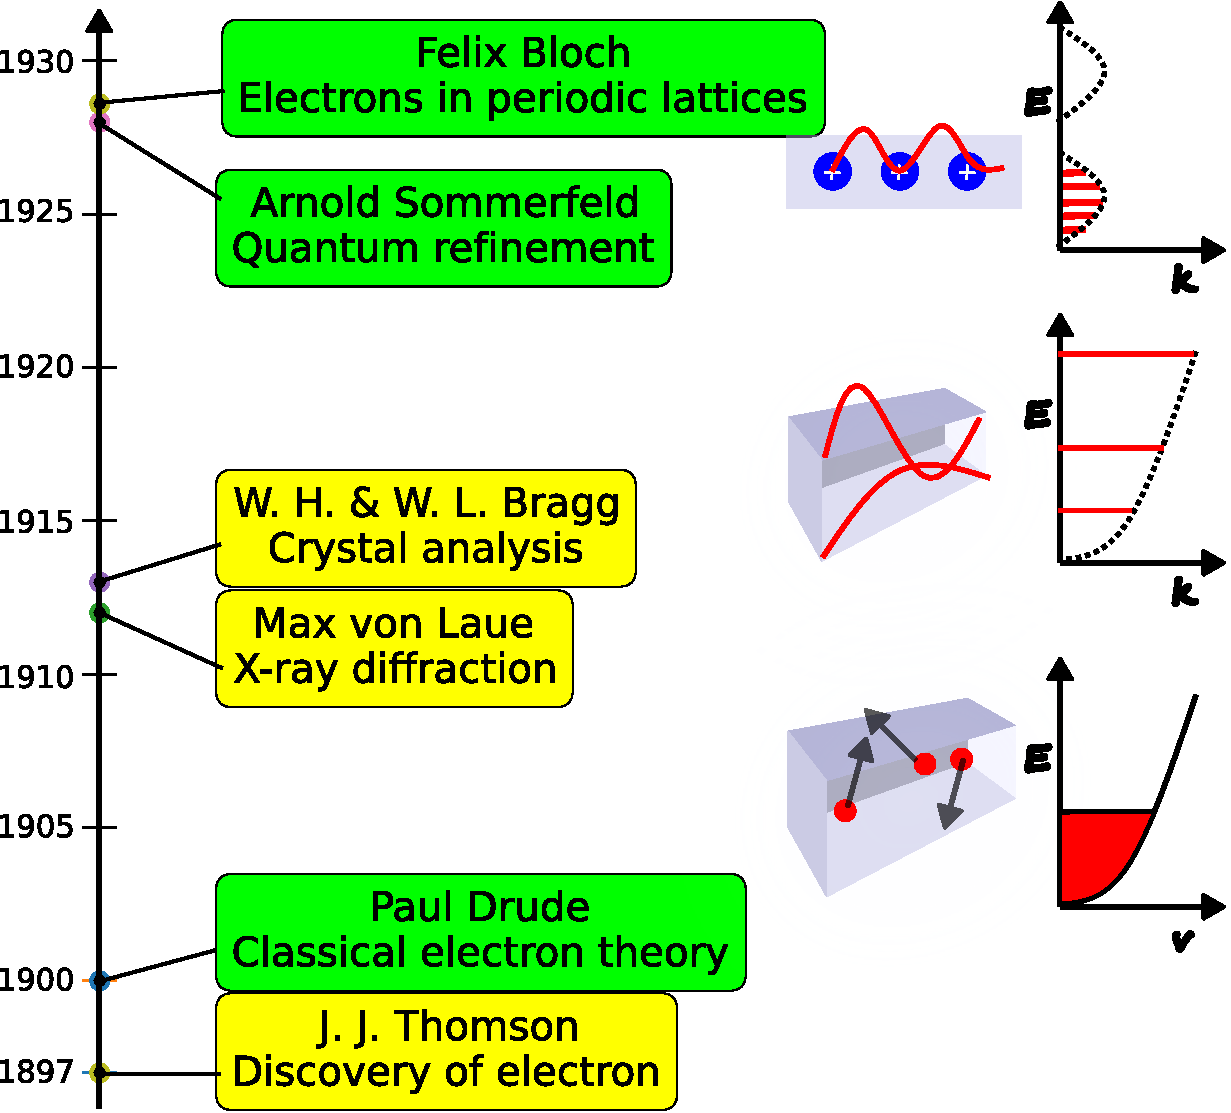
\includegraphics[width=\textwidth]{metals_discovery_timeline}
		\end{figure}
	\end{column}
\end{columns}
\end{frame}
%

	%\fi
	%
	\section{Classical free electron theory}
	%
	%\ifshowhidden
	%
\againframe{plan}
%
\begin{frame}{Problem at hand}
	%
	\begin{figure}
		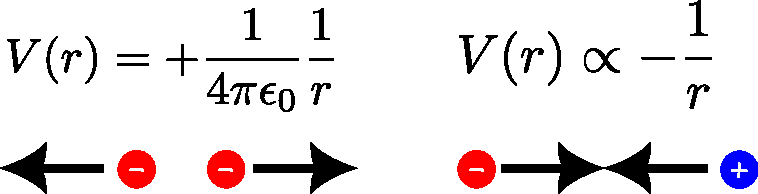
\includegraphics[width=0.8\textwidth]{metals_coulomb_force}
	\end{figure}
	\begin{itemize}
		\item The problem at hand is to solve the motion of interacting particles-- electrons of the order of \num{e23} and ions of the order of \num{e23}.
		\item This is a tough problem. The idea is to simplify the problem by making \textbf{approximations}.
	\end{itemize}
	%
\end{frame}
\begin{frame}{Classical free electron theory}
	%
	\begin{columns}
		\begin{column}[t]{0.85\textwidth}
			\begin{itemize}
				\item Ohm's law was discovered in 1827 and needed explanation.
				\item Proposed by Paul Drude in 1900 using analogy of gas of molecules.
				\item Mutual repulsion between electrons is neglected i.e. electrons are independent -- \textbf{independent electron approximation}. 
				\item Assumed ``gas'' is \textbf{free} i.e. not under influence of  lattice --  \textbf{free electron approximation}

				\item Role of lattice is to redistribute the velocity distribution that obeys \textbf{classical} Maxwell-Boltzmann statistics --  classical thermodynamics.
				\item \fcolorbox{green}{white}{The theory explains Ohm's law}
				\item Hendrik Lorentz extended theory to explain thermal conductivity -- hence Drude-Lorentz electron theory.
			\end{itemize}
		\end{column}
		%
		\begin{column}[t]{0.13\textwidth}
			\begin{figure}
				\centering
				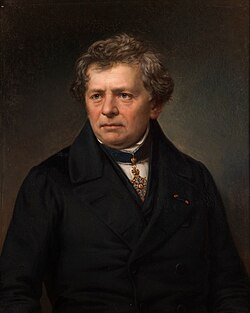
\includegraphics[width=0.9\textwidth]{Georg_Simon_Ohm_1789_1854}
				\\
				{\centering\footnotesize G. Ohm}
				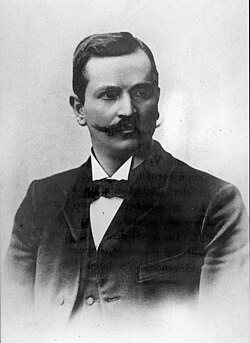
\includegraphics[width=0.9\textwidth]{Paul_Drude_1863_1906}
				\\
				{\centering\footnotesize P. Drude}
				\begin{overpic}[width=0.9\textwidth]{Hendrik_Lorentz_1853_1928}
					% Overlay image on top
					\put(0,0){\includegraphics[width=0.4\textwidth]{Alfred_Nobel_1833_1896}}
				\end{overpic}
				\\
				{\centering\footnotesize H. Lorentz }
			\end{figure}
		\end{column}
	\end{columns}
\end{frame}
%
%
\begin{frame}{Independent electron approximation}
	%
\begin{figure}
	\centering
	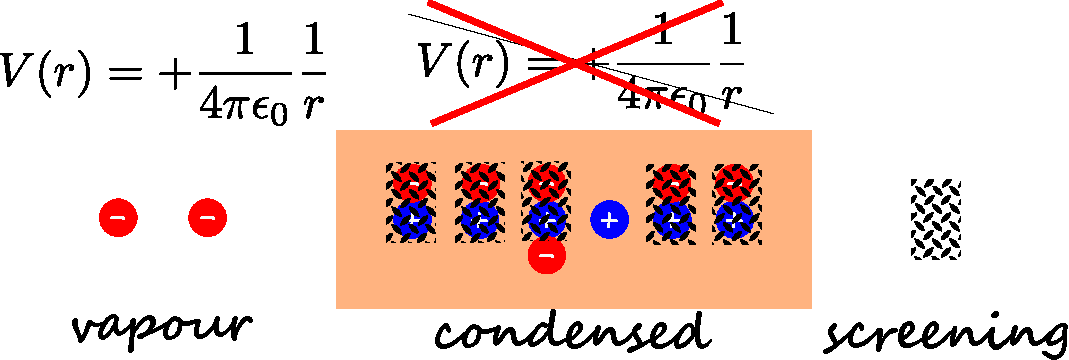
\includegraphics[width=0.6\textwidth]{metals_independent_electron_approximation}
\end{figure}
	\begin{itemize}
	\item In the condensed phase, there are of the order of \num{e23} electrons.
	\item The repulsive Coulomb potential between an electron and other electron is \textbf{screened} due to large numbers and results in an \textbf{independent} electron.
	\item The problem of motion of \(\mathcal{O}(\num{e23})\) electrons is reduced to the problem of motion of \textbf{single} electron.
\end{itemize}
%
\begin{keyinsight}
	The property of single electron determines the properties of electron gas.
\end{keyinsight}
\end{frame}
\begin{frame}{Free electron approximation}
	%
	\begin{figure}
		\centering
		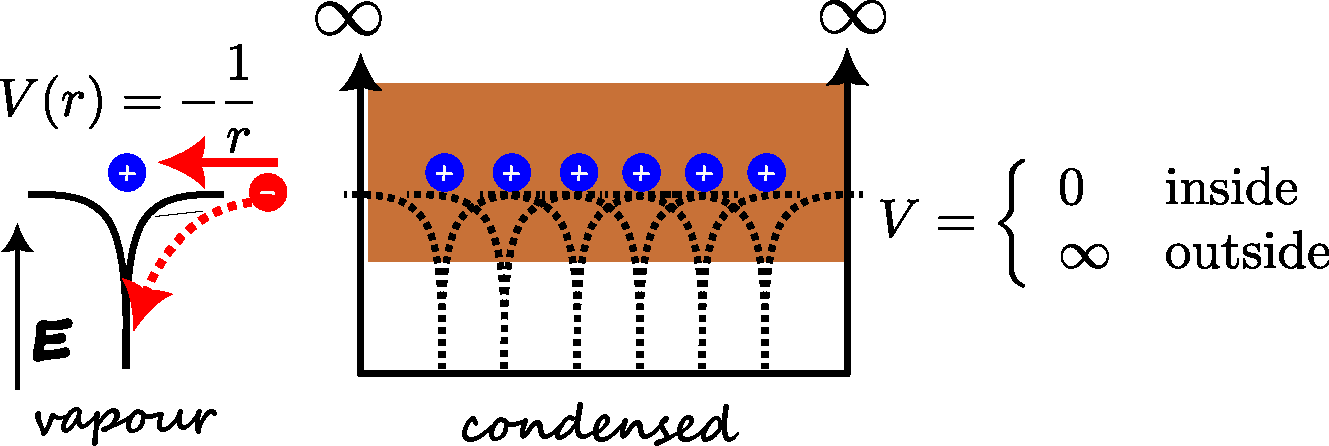
\includegraphics[width=0.6\textwidth]{metals_free_electron_approximation}
	\end{figure}
	\begin{itemize}
		\item The attractive Coulomb potential between ions and an electron is smeared due to large numbers and results in constant potential in the interior of metal with \textbf{infinite} barrier at the surface. This potential is called \textbf{infinite potential well}.
		\item This potential traps the electrons analogous to gas atoms in a container.
		\item The electrons are free to move in the potential well. The kinetic energy \(K\) of an electron with mass \(m\) and velocity \(\vb{v}\) is
		\[
		K = \frac{1}{2}m v^2
		\]
	\end{itemize}
\end{frame}
%
\begin{frame}{Classical thermodynamics}
	%
\begin{figure}
	\centering
	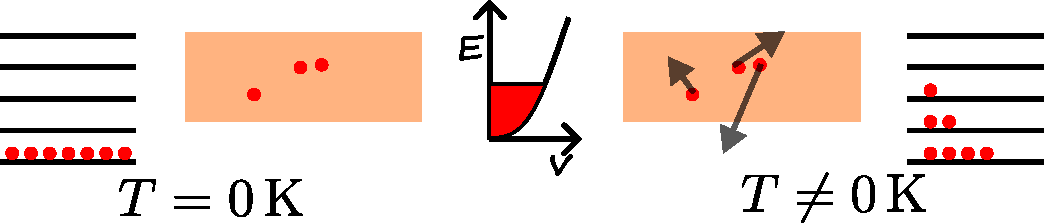
\includegraphics[width=\textwidth]{metals_classical_thermodynamics}
\end{figure}
\begin{columns}
	\begin{column}[t]{0.85\textwidth}
\begin{footnotesize}
			\begin{itemize}
	\item At temperature \(T=0\), electrons are frozen. At \(T\neq0\), due to the large number of electrons and collisions, the kinetic energy of electrons keeps changing.
	\item However, the probability to find electron with with lower energy is higher than the probality to find electron with higher energy. This is the essence of Maxwell-Boltzmann statistics.
	\item The average kinetic energy \(\langle T \rangle\) at temperature is 
	\[
	\langle K \rangle = \frac{3}{2} k_B T,
	\]
	where \(k_B\) is the Boltzmann constant.
\end{itemize}
\end{footnotesize}
	\end{column}
	%
	\begin{column}[t]{0.13\textwidth}
			\begin{figure}
			\centering
			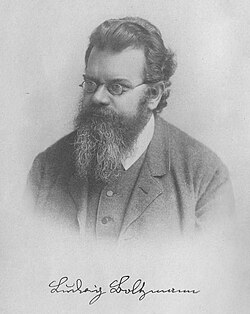
\includegraphics[width=0.9\textwidth]{Maxwell_Boltzmann_1844_1906}
			\\
			{\centering\footnotesize Boltzmann}
			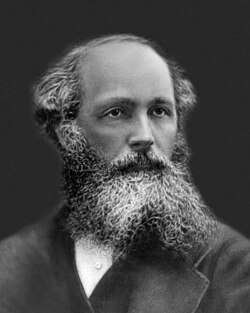
\includegraphics[width=0.9\textwidth]{James_Clerk_Maxwell_1831_1879}
			\\
			{\centering\footnotesize Maxwell}
		\end{figure}
	\end{column}
\end{columns}
\end{frame}
\begin{frame}{Classical free electron theory}
	%
	\begin{figure}
		\centering
		\href{run:images/electron_drift_lattice_animated_drude_electron_without_electric_field.gif}{%
			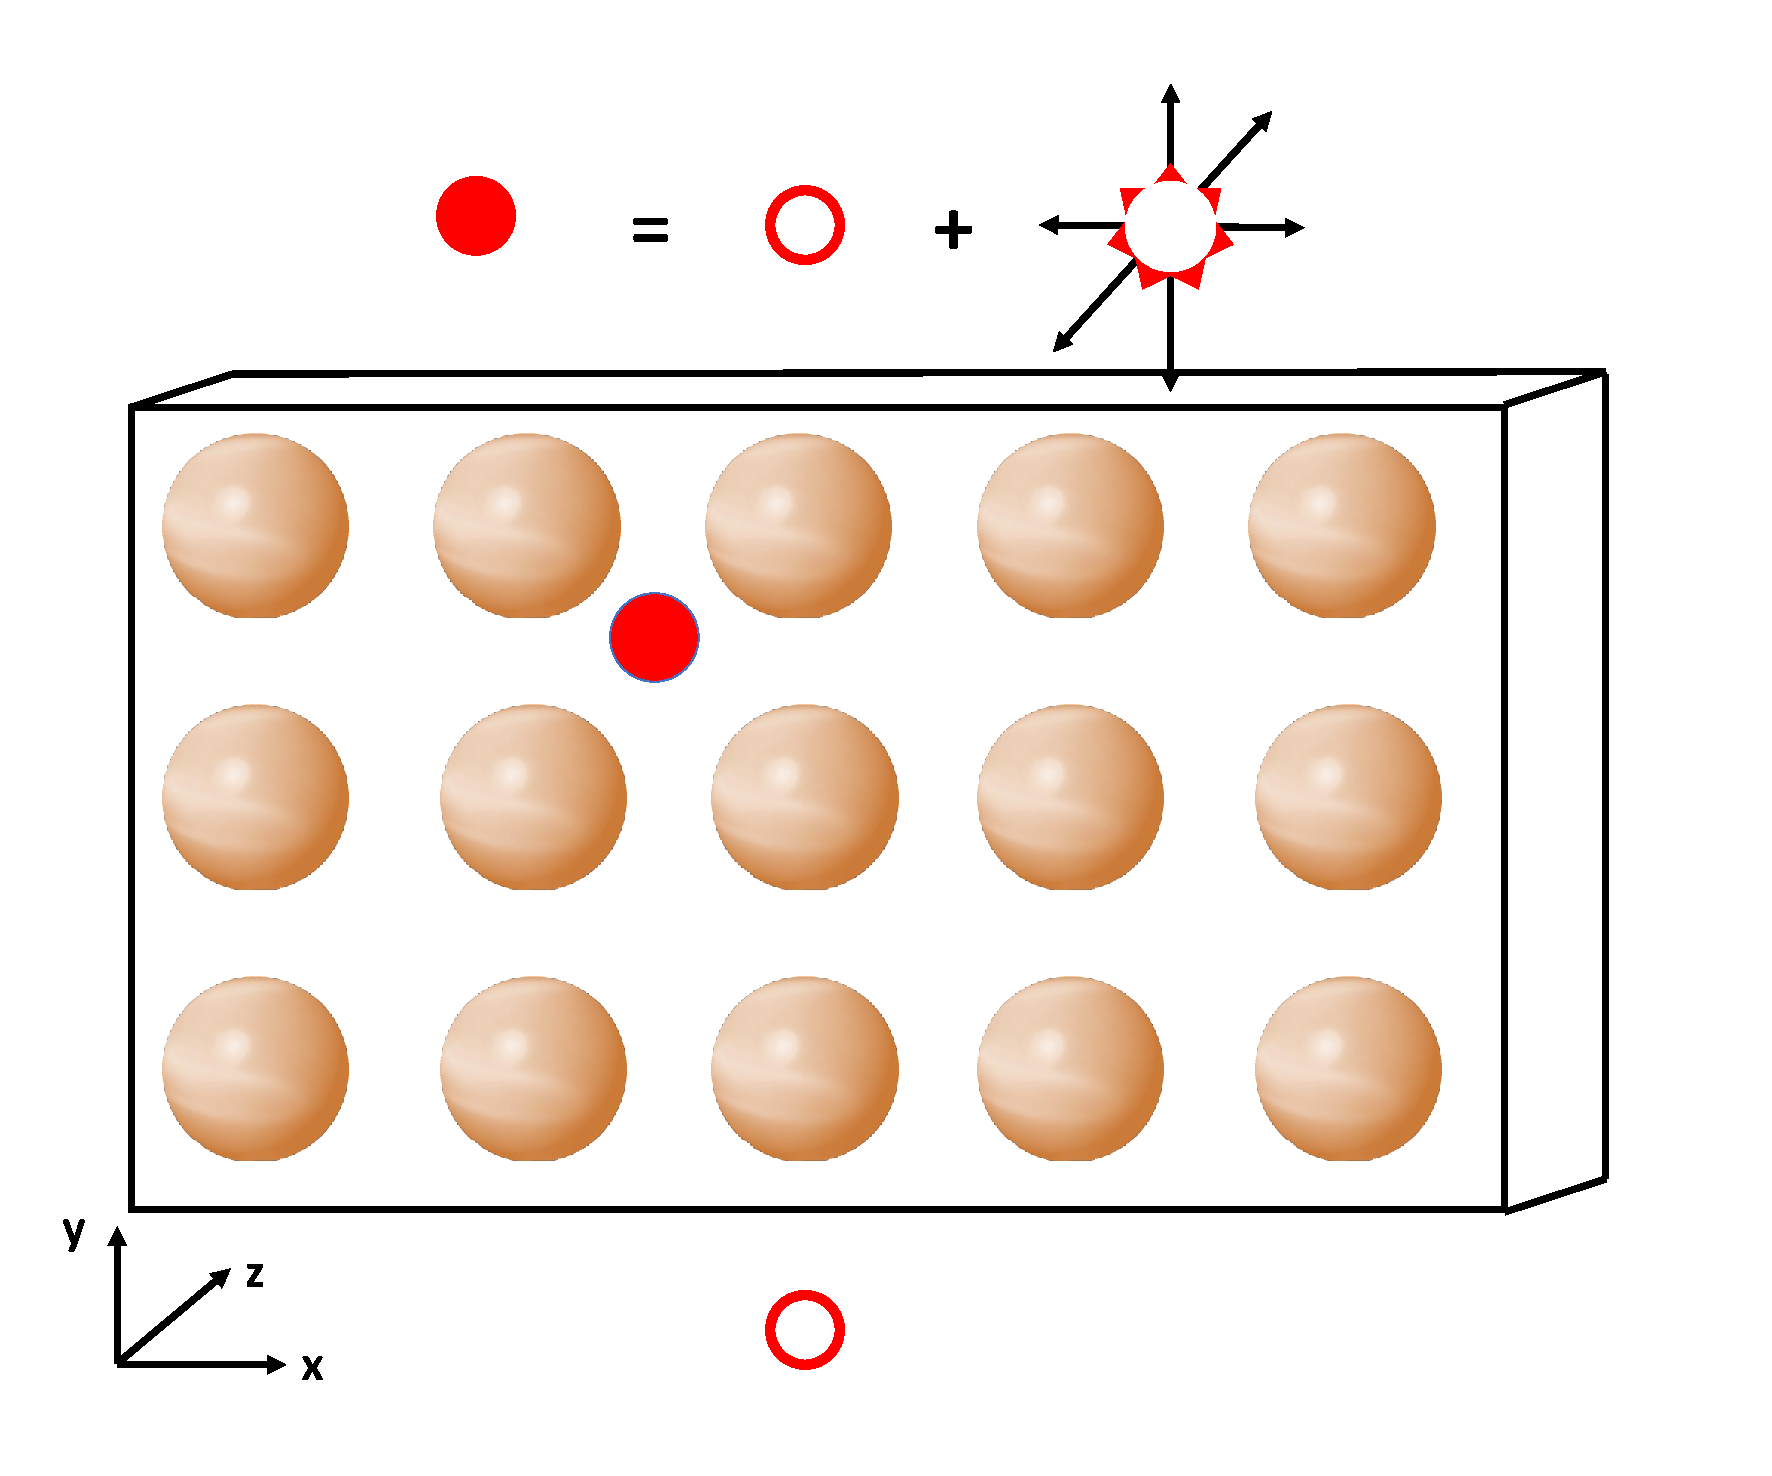
\includegraphics[width=0.4\textwidth]{electron_drift_lattice_animated_drude_electron_without_electric_field}%
		}
	\end{figure}
	%
	\begin{itemize}
		\item Electron motion is decomposed into \textbf{thermal motion} and \textbf{drift motion}.
		\item Thermal motion is due to random collisions with the lattice. 
		\item Drift motion is the net motion of electrons. The electron drifts only between collisions.
	\end{itemize}
	%
\end{frame}
%
\begin{frame}{Thermal motion}
	\begin{definition}
		Mean free path \(l_{mf}\) is defined as the average distance the electron travels between collisions.
	\end{definition}
	\begin{definition}
		Thermal velocity \(v_{th}\) is defined as the average velocity of the electron.
	\end{definition}
	%
	\begin{itemize}
		\item Thermal motion has two properties mean free path \(l_{mf}\) and thermal velocity \(v_{th}\).
		\item Drude assumed that \(l_{mf}\) is a material constant.
		\item At room temperature (\SI{~300}{\kelvin}), the thermal velocity is of the \textbf{order of \SI{e5}{\metre\per\second}}.
	\end{itemize}
	%
	\begin{guesstimate}{Average kinetic energy of electron}
		Take room temprerature as \SI{27}{\celsius}. Express energy in \si{\electron\volt}. \hfill [Hint: \SI{1}{\electron\volt} = \SI{1.602e-19}{\joule}]
	\end{guesstimate}
\end{frame}
%
\begin{frame}{Drift motion}
		\begin{itemize}
		\item In the absence of external force, the drift motion is zero.
		\item The external force \(\vb{F}_{ext}\) on the electron is given by the Lorentz force
		\[
		\vb{F}_{ext} = -e \vb{E} -e \vb{v}\times\vb{B},
		\]
		where \(\vb{E}\) is the electric field and \(\vb{B}\) is the magnetic field.
		\item The effect of the collisions is treated as a drag or frictional force
		\[
		\vb{F}_{fric} = -m \frac{\vb{v}}{\tau}.
		\] 
		\item Since Lorentz extended the theory to incorporate electromagnetic force, the theory is also the Lorentz-Drude theory.
	\end{itemize}
\end{frame}
%
\begin{frame}{Lorentz-Drude theory -- Postulates}
	\begin{block}{Postulates}
		\begin{enumerate}
			\item \textbf{Particles:} Electrons are \textbf{classical} particles with mass \(m\) and charge \(-e\).
			\item \textbf{Kinematics:} 
			\begin{itemize}
				\item \textbf{Independent electron approximation:} Electrons are independent and mutual repulsion between them is ignored.

			\end{itemize}
			\item \textbf{Dynamics:} 
			\begin{itemize}
				\item \textbf{Free electron approximation:} Electrons are free and move in an \textbf{infinite potential well}.
				\item \textbf{Thermal motion:} Electron undergoes \textbf{random} collision with ion cores. Random collisions lead to thermal motion.
				\item \textbf{Drift motion:} In between collisions, the Lorentz force acts on electron and leads to drift motion.
			\end{itemize}
			\item \textbf{Classical Thermodynamics:} The average electron energy is given by Maxwell-Boltzmann statistics. 
		\end{enumerate}
	\end{block}
	%
\end{frame}
%
%------------------------
\begin{frame}{Ohm's law}
	\begin{figure}
		\centering
		\href{run:images/electron_drift_lattice_animated_drude_electron_with_electric_field.gif}{%
			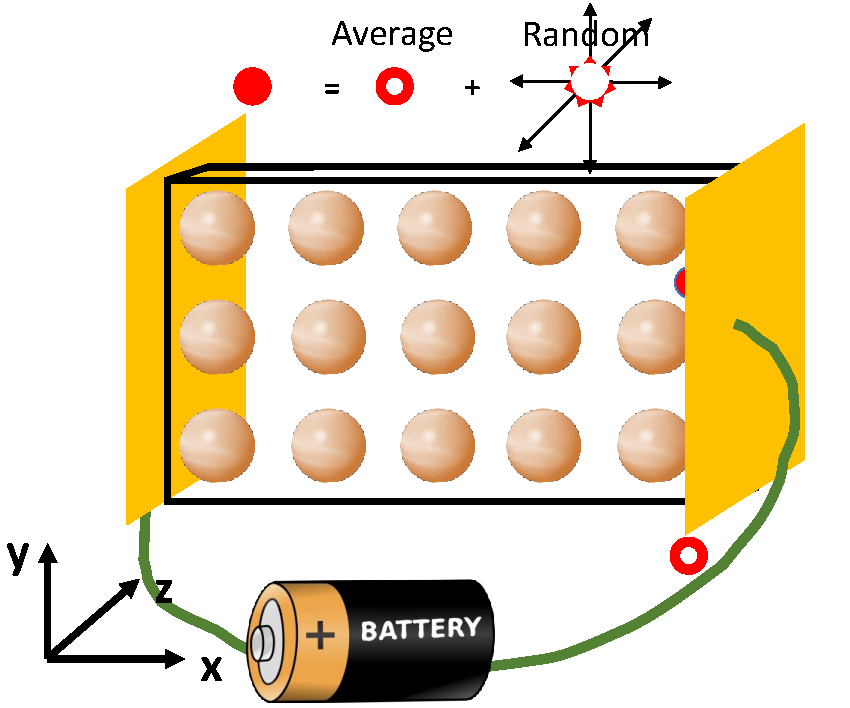
\includegraphics[height=0.4\textheight]{electron_drift_lattice_animated_drude_electron_with_electric_field}%
			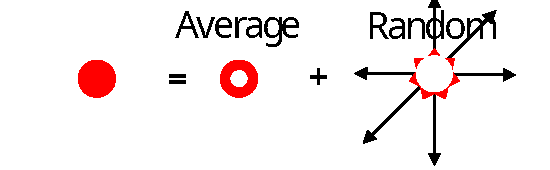
\includegraphics[height=0.2\textheight]{metals_electron_motion_decomposition}
		}
	\end{figure}
	%
	\begin{itemize}
		\item The motion of electron is decomposed into an \textbf{average} part and the \textbf{random} part.
		\item The average part ``drifts'' with a constant velocity under electric field. The random part has \textbf{zero} net motion.
	\end{itemize}
	\begin{learningobjectives}
		Classical electron theory explains Ohm’s law qualitatively.
	\end{learningobjectives}
\end{frame}
%
\begin{frame}{Ohm's law: Macroscopic version}
	%
	\begin{minipage}[t]{0.7\textwidth}
		\begin{itemize}
			\item The \textbf{macroscopic} version of the Ohm's law states that potential \(V\) applied across a metal is directly proportional to the current \(I\) flowing across it. The constant of proportionaly is called the resistance \(R\).
			\item Its \textbf{microscopic} version relates the electric field and current density
			\item Electric field \(\vb{E}\) is defined as the potential per unit distance. Its SI unit is \si{\volt\per\metre}.
			\item Current density \(\vb{j}\) is defined as the current flowing through a wire per unit area,
			
			where \(A\) is the cross-sectional area of the wire. Its SI unit is \si{\ampere\per\metre\squared}.
		\end{itemize}
	\end{minipage}
	%
	\begin{minipage}[t]{0.28\textwidth}
		\[
		V = IR
		\]
		%\vspace{10ex}
		\begin{figure}
			\centering
			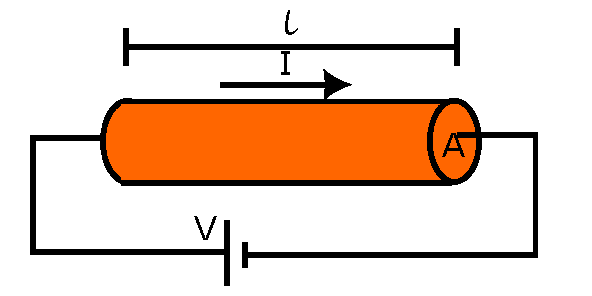
\includegraphics[width=\textwidth]{metals_ohms_law_derivation}
		\end{figure}
		%
		\vspace{3ex}
		\[
		\vb{E} = \frac{V}{\ell}\vu{E}
		\]
		\[
		\vb{j} = \frac{I}{A}\vu{j}
		\]
	\end{minipage}
	%
\end{frame}
%
\begin{frame}{Ohm's law : Microscopic version}
	%
	Lets start with the macroscopic version \(V = R I\) and derive the microscopic version of Ohm's law
	\begin{derivation}
		%
		Upon substitution of \(V, I\) in terms of \(\vb{E}, \vb{j}\), we have
		\[
		\frac{\ell}{V} \vb{E} = \frac{A}{I} \vb{j}
		\quad \Rightarrow \quad
		\vb{j} = \frac{\ell}{A} \frac{I}{V} \vb{E}
		\quad \Rightarrow \quad
		\vb{j} = \frac{\ell}{A R} \vb{E} = \sigma \vb{E}
		\]
		Thus, the microscopic version of Ohm's law is given by
		\begin{center}
			\framebox{$\vb{j} = \sigma \vb{E}$}
		\end{center}
		%
		where \(\sigma\) is given by
		\[
		\sigma = \frac{\ell}{A R}
		\]
	\end{derivation}
\end{frame}
%
\begin{frame}{Conductivity -- \(\sigma\)}
	%
	\begin{definition}
		The conductivity \(\sigma\) is defined as the current density carried by the wire per unit of electric field.
		\[
		\sigma = \frac{j}{E}
		\quad\quad
		\text{SI unit}
		\quad 
		[\sigma] = \left[ \frac{\ell}{A R}\right] = \text{\si{\per\ohm\per\metre}}.
		\]
	\end{definition}
	%
	\begin{question}
		A copper wire of length \(L=\) \SI{2}{\metre} and diameter \(d\)=\SI{1}{\milli\metre} is connected across a DC source. When a voltage of \(V\)=\SI{0.5}{\volt} is applied across the ends of the wire, an electric current of \(I\)=\SI{22}{\ampere} is observed.
		Using these measurements, find the electrical conductivity \(\sigma\) of copper.
	\end{question}
	%
	\begin{keyinsight}
		Metals have high conductivity.
	\end{keyinsight}
\end{frame}
%------------------------
\begin{frame}{Applications of metallic conductivity}
	%
	Due to high conductivity, metals have many applications ranging from power electronics to microelectronics, from mechanical to aerospace industry.
	\begin{figure}
		\centering
		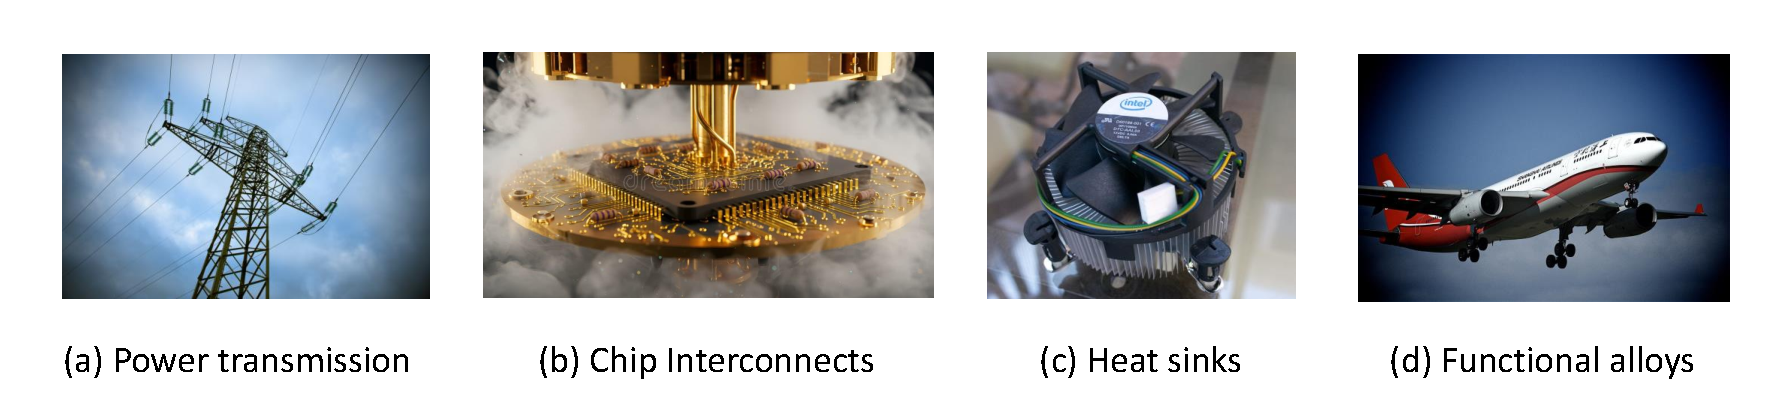
\includegraphics[width=\textwidth]{metals_applications}
	\end{figure}
	\begin{itemize}
		\item Power transmission: Copper/Aluminum cables.
		\item Electronic devices: Contacts, interconnects.
		\item Thermal applications: Heat sinks, cookware.
		\item Alloys: Enhanced strength and corrosion resistance.
	\end{itemize}
\end{frame}

%------------------------
\begin{frame}{Summary of Lecture}
	\begin{itemize}
		\item Materials are classified into conductors, semiconductors, and insulators.
		\item Metals have high conductivity due to free electrons.
		\item Drude's classical electron theory introduced microscopic picture of conduction.
		\item Conductivity is related to resistivity.
	\end{itemize}
\end{frame}
%
\begin{frame}{Materials: Beyond metals}
\begin{tiny}
		\begin{table}
		\centering
		\begin{tabular}{c c c c c c c}
			\toprule
			Condensed	&	Elec.	&	Therm.	&	Opt.	&	Ductile		&	Material	&	Application			\\
			\midrule
			Solid	&	\(\Uparrow\)	&	-	&	-	&	\(\downarrow\)	& Superconductor	&	Levitation\\
			Solid	&	\(\Downarrow\)	&	\(\Uparrow\)	&	-	&	-		& Diamond	&	Chips \\
			Liquid	&	\(\Downarrow\)	&	\(\Uparrow\)	&	-	&	-		& Dielectric coolants	&	Heatsinks \\
			\bottomrule
		\end{tabular}
		\caption{New materials with mixed properties.}
	\end{table}	
\end{tiny}
%
\begin{figure}
	\centering
	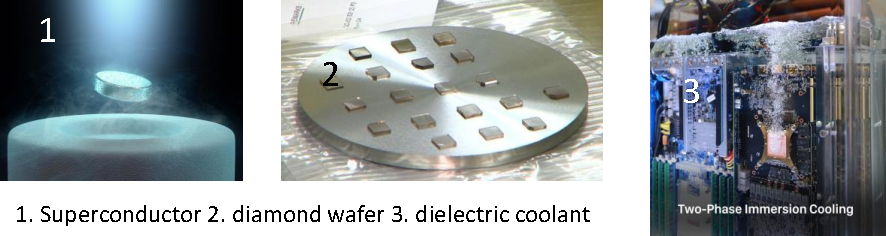
\includegraphics[width=\textwidth]{metals_beyond_metals}
\end{figure}
\end{frame}
	%\fi
	%
	\section{Expression of electrical conductivity}
	%
	%\ifshowhidden
	%
\againframe{plan}
%
\begin{frame}{Lecture plan}
	\begin{learningobjectives}
		\begin{itemize}
			\item From qualitative picture of metals to quantitative derivation.
			\item Derive expression for conductivity.
			\item Mobility is a material property.
		\end{itemize}
	\end{learningobjectives}
\end{frame}
%
%
\begin{frame}{Free electron density -- \(n\)}
	\begin{block}{Definition}
		\begin{itemize}
			\item Electron density \(n\) is defined as the number of electrons per unit volume. Its SI unit is \si{\per\metre\cubed}.
			\item For metals, each atom contributes as many electrons as its \textbf{valency}. For example, \ce{Na} has valency 1.
		\end{itemize}
	\end{block}
	\begin{guesstimate}{Electron density of metals}
		%
		\begin{enumerate}\itemsep0pt\parskip0pt \parsep0pt
			\item Take the radius \(r_s\) of atom is nearly $3 a_0$, where \(a_0 =\)~\SI{0.529}{\angstrom} is the Bohr radius.
			\item Deduce \(n\) is of the order \SI{e22}{\per\centi\metre\cubed} =  \SI{e28}{\per\metre\cubed}.
			\item For Cu, the experimental observed \(n\)~=\SI{8.47e28}{\per\metre\cubed}.
		\end{enumerate}
	\end{guesstimate}
	%
	\vfill
	\begin{keyinsight}
		\(\tfrac{r_s}{a_0}\) determines the free electron density.
	\end{keyinsight}
	%
\end{frame}
%
\begin{frame}{Drift velocity -- \(v_d\)}
	\begin{minipage}{0.7\textwidth}
		\begin{definition}
			\begin{itemize}
				\item \textbf{Drift velocity} \(\vb{v_d}\)is defined as the average velocity of an electron in the presence of electric field.
				\item \textbf{relaxation time} $\tau$ is defined as the average time between collisions.
			\end{itemize}
		\end{definition}
	\end{minipage}
	\begin{minipage}{0.28\textwidth}
		\begin{figure}
			\centering
			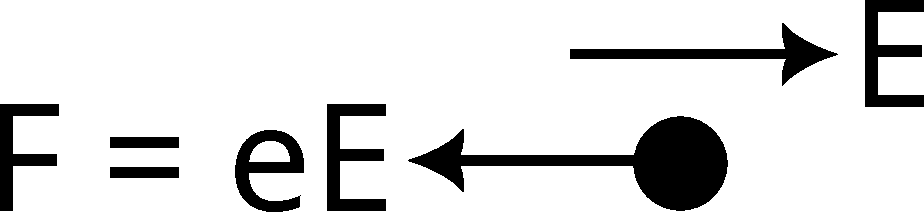
\includegraphics[height=0.05\textheight]{metals_drift_equation}
		\end{figure}
	\end{minipage}
	\begin{derivation}
		\begin{minipage}[t]{0.6\textwidth}
			\begin{itemize}
				\item The equation of motion of electron is
				\item During time duration \(\tau\), electron reaches drift velocity
			\end{itemize}
		\end{minipage}
		%
		\begin{minipage}[t]{0.38\textwidth}
			\[
			\vb{a} = -\frac{e}{m} \vb{E}
			\]
			\[		
			\framebox{
				$
				\vb{v_d} = -\frac{e\tau}{m}\vb{E}
				$}
			\]
		\end{minipage}
	\end{derivation}
	\begin{keyinsight}
		Drift velocity is proportional to the applied electric field.
	\end{keyinsight}
\end{frame}
%
\begin{frame}{\(y=mx\) and \(y= m /x\) relations}
	\begin{itemize}
		\item We have seen many examples of \textbf{linear} relations between physical quantities till now.
		\item The dependent variable \(y\) relates to the independent variable \(x\). The relation is given by the \textbf{constant of proportionality}.
		\item We also say that ``\(y\) is directly proportional to \(x\)''.
	\end{itemize}
	%
{
	%\small
		\begin{table}
		\centering
		\begin{tabular}{l c l}
			\toprule
			Law 	&	Equation 	&	Const. of prop.	\\
			\midrule
			Ohm's (macroscopic)	&	\(I = \frac{1}{R} V\)	&	Conductance	\\
			Ohm's (microscopic)	&	\(\vb{j} = \sigma \vb{E}\)	&	Conductivity \\
			Capacitor			&	\(E = \frac{1}{d} V\)	&	1/Separation	\\
			Drift motion			&	\(\vb{v_d} = -\frac{e \tau}{m} \vb{E}\)		&	Mobility	\\
			Photoelectric effect	&	\(	E = \hbar \nu\)	&	Planck's constant	\\
			\bottomrule
		\end{tabular}
	\end{table}
}
\end{frame}
%
\begin{frame}{\(y=mx\) and \(y= m /x\) relations contd...}
	%
		%
	\begin{itemize}
		\item Sometimes, physical quantities are also inversely related i.e. \(y \propto \tfrac{1}{x}\).
		\item We also say ``y is inversely proportional to x''.
	\end{itemize}
	%
	{
		%\small
		\begin{table}
			\centering
			\begin{tabular}{l c l}
				\toprule
				Law 	&	Equation 	&	Const. of prop.	\\
				\midrule
				Light	&	\(\nu = c\frac{1}{\lambda}\)	&	velocity	\\
				\bottomrule
			\end{tabular}
		\end{table}
	}
	%
\end{frame}
\begin{frame}{Mobility -- \(\mu\)}
	%
	\begin{definition}
		\textbf{Mobility} \(\mu\) is defined as the drift velocity per unit electric field
		\[
		\mu = \frac{v_d}{E}.
		\]
	\end{definition}
	%
	\begin{itemize}
		\item It is a material property as
		\[
		\mu = \frac{e\tau}{m} \qquad \qquad [\because \vb{v_d} = -\frac{e\tau}{m}\vb{E}]
		\]
		\item Its SI unit is
		\[
		[\mu] = \frac{[v_d]}{[E]} = \frac{[v_d \ell]}{[V]} = \text{\si{\metre\squared\per\volt\per\second}}
		\]
	\end{itemize}
	%
\end{frame}
%
\begin{frame}{Conductivity \(\sigma\)}
	%
	\begin{minipage}{0.28\textwidth}
		\begin{figure}
			\centering
			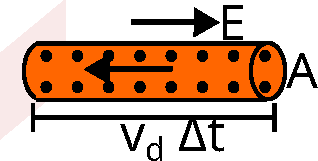
\includegraphics[width=\textwidth]{metals_conductivity_expression}
		\end{figure}
	\end{minipage}
	%
	\begin{minipage}{0.7\textwidth}
		In a time duration \(\Delta t\), the number of electrons \(N\) in a volume of \(V = v_d \Delta t A\) will pass through the cross section of area \(A\).
	\end{minipage}
	%
	\begin{small}
		\begin{derivation}
			%
			\begin{minipage}[t]{0.3\textwidth}
				\begin{enumerate}
					\item Current \(I\):
					\item Current density \(j\):
					\item Conductivity \(\sigma\):
				\end{enumerate}
			\end{minipage}
			\begin{minipage}[t]{0.68\textwidth}
				\vspace*{0pt} % forces content to start at top
				\begin{align}
					I &= -\frac{Ne}{\Delta t} =  -\frac{n\cdot V}{\Delta t} = - nev_d  A	\\
					%
					j &= \frac{I}{A} = -ne v_d = \dfrac{ne^2\tau}{m}E	\\
					%
					\sigma &= \dfrac{ne^2\tau}{m} = ne\big(\dfrac{e\tau}{m}\big) = ne\mu
				\end{align}
				
			\end{minipage}
		\end{derivation}
	\end{small}
	%
	\begin{learningobjectives}
		We have derived the expression for conductivity.
	\end{learningobjectives}
\end{frame}
%
\begin{frame}{Relaxation Time -- \(\tau\)}
	%
	\begin{block}{Assumption}
		Relaxation time \(\tau\) is assumed to be a \textbf{constant}.
	\end{block}
	\begin{guesstimate}{Relaxation time in metals}
		Estimate the electron relaxation time in metals.
		\begin{enumerate}\itemsep0pt\parskip0pt \parsep0pt
			\item Take conductivity \(\sigma \sim\)~\SI{e7}{\siemens\per\metre}, number density \(n \sim\)~\SI{e28}{\per\metre\cubed}
			\item Take electron mass  \(m\)~=\SI{9.1e-31}{\kilo\gram}, charge \(e\)~=\SI{1.609e-19}{\coulomb}.
			\item Deduce relaxation time \( \tau \sim\)~ \framebox{\SI{e-14}{\second} or \SI{10}{\femto\second}}.
		\end{enumerate}
	\end{guesstimate}
	\begin{itemize}
		\item Larger $\tau$ → fewer collisions → higher conductivity.
	\end{itemize}
	%
	\begin{trends}
		\begin{enumerate}\itemsep0pt\parskip0pt \parsep0pt
			\item As temperature increases, \(\tau\) decreases. \hfill Why?
			\item As impurity concentration increases, \(\tau\) decreases. \hfill Why?
		\end{enumerate}
	\end{trends}
\end{frame}
%
\begin{frame}{Resistivity -- \(\rho\)}
	\begin{definition}
		Resistivity \(\rho\) is defined as the inverse of conductivity
		\[
		\rho = \frac{1}{\sigma}
		\]
		Its SI unit is \si{\ohm\metre}.
	\end{definition}
	\begin{itemize}
		\item Resistivity $\rho = \dfrac{1}{\sigma} = \dfrac{m}{ne^2\tau}$.
		\item Its SI unit is \si{\ohm\metre}.
	\end{itemize}
	%
	\begin{trends}
		\begin{enumerate}\itemsep0pt\parskip0pt \parsep0pt
			\item As number density increases, $\rho$ decreases. \hfill Why?
			\item As temperature increases, $\rho$ increases. \hfill Why?
		\end{enumerate}
	\end{trends}
\end{frame}
%
\begin{frame}{Summary of physical quantities}
	\begin{table}
		\centering
		\begin{tabular}{l c c c}
			\toprule
			Physical quantity	&	Symbol	& Units	& Material Property	\\
			\midrule
			Resistance	&	\(R\)	&	\si{\ohm}	&	No	\\
			Conductivity	& \(\sigma\)	&	\si{\per\ohm\per\metre} or \si{\siemens\per\metre}	&	Yes	\\
			Mobility	&	\(\mu\)	&	\si{\metre\squared\per\volt\per\second}	&	Yes 	\\
			Relaxation Time	&	\(\tau\)	&	\si{\second}	& Yes	\\
			Resistivity	&	\(\rho\)	&	\si{\ohm\metre}	&	Yes	\\
			\bottomrule
		\end{tabular}
	\end{table}
\end{frame}
%
\begin{frame}{Theory vs. experiment}
	%
	\begin{block}{\textcolor{green}{Merit: Conductivity order of magnitude}}
		\begin{itemize}
			\item For metals, classical free electron theory (CEFT) predicts order of magnitude of conductivity correctly.  
			\[\sigma_{\mathrm{experiment}} \sim \sigma_{\mathrm{theory}} \sim \SI{e7}{\per\ohm\per\metre} \]
		\end{itemize}
	\end{block}
	%
	%
	\begin{block}{\textcolor{red}{Demerit: Conductivity vs valency}}
		\begin{itemize}
			\item Conductivity is proportional to number density. Number density is proportional to valency. So theory predicts conductivity increases with valency. But experiment shows monovalent metals (\ce{Na}, \ce{K}) have higher conductivity than divalent metals (\ce{Mg}, \ce{Ca}).
		\end{itemize}
	\end{block}
\end{frame}
%
\begin{frame}{Theory vs Experiment contd...}
	\begin{block}{\textcolor{red}{Demerit: Hall coefficient sign}}
		\begin{itemize}
			\item In metals, there are only electrons as charge carriers.
			\item It is expected that the \textbf{sign of Hall coefficient is negative}.
			\item However, experiments show metals like \ce{Zn} show positive Hall coefficient. CEFT cannot explain this \textbf{anomaly}.
		\end{itemize}
	\end{block}
	%
	\begin{block}{\textcolor{red}{Under-estimation of mean free path}}
		\begin{itemize}
			\item The mean free path is considered a constant in CEFT and is taken as the interatomic distance that is approximately \SI{5}{\angstrom}.
			\item However, experiment shows mean free path to be of the order \SI{50}{\angstrom}.
			\item Thus, CEFT underestimates the mean free path by one order of magnitude.
		\end{itemize}
	\end{block}
\end{frame}
\begin{frame}{\textcolor{red}{Demerit: Classification of materials}}
		%
		\begin{figure}
			\centering
			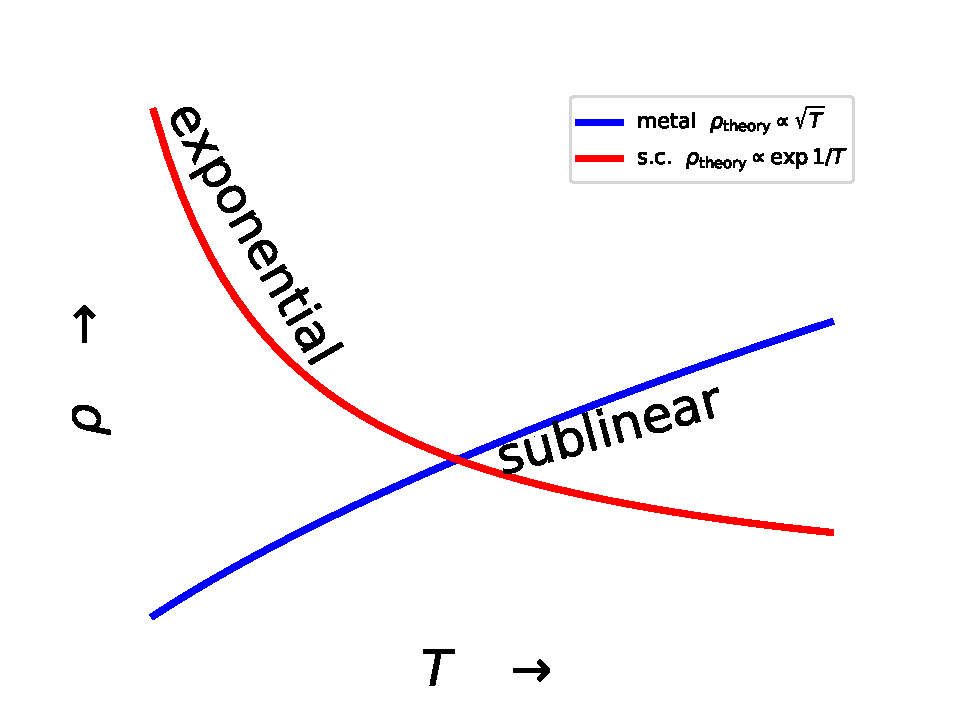
\includegraphics[width=0.7\textheight]{metals_semiconductors_resistivity}
		\end{figure}
		%
		\begin{itemize}
			\item CEFT \textbf{does not} explain the classification of materials into conductors, semi-conductors and insulators.
			\item For example, the resistivity of metals varies linearly
			\(
			\rho_\mathrm{conductor} \propto T
			\)
			but resistivity of semiconductors varies exponentially
			\(
			\rho_\mathrm{semi-conductor} \propto \exp(\frac{1}{T}).
			\)
		\end{itemize}
\end{frame}
%
\begin{frame}{\textcolor{red}{CFET Demerit: Resistivity vs temperature}}
	%
	\begin{figure}
		\centering
		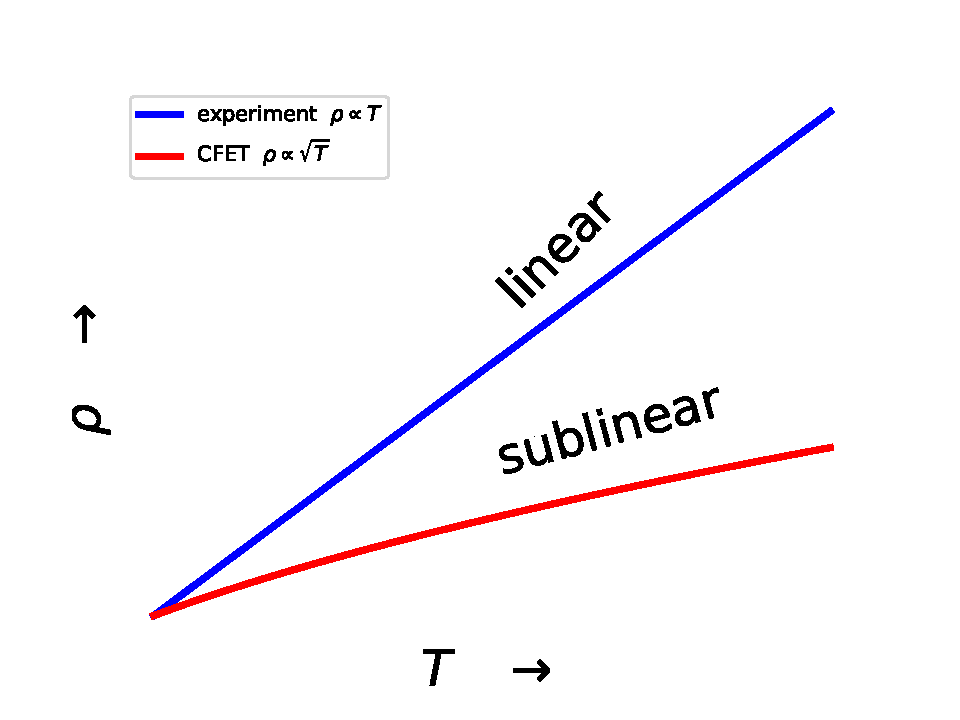
\includegraphics[width=0.8\textheight]{metals_resistivity_theory_vs_experiment}
	\end{figure}
	%
	\begin{itemize}
		\item Wrong prediction of temperature dependence of conductivity. Theory predicts
		\(
		\sigma(T) \propto 1/\sqrt{T},
		\) 
		but experimental trend is
		\(
		\sigma(T) \propto T^{-1}.
		\)
	\end{itemize}
\end{frame}
%
\begin{frame}{\textcolor{red}{Demerit: Specific heat capacity}}
\begin{footnotesize}
		\begin{itemize}
		\item Metals heat ``quickly''. When we heat a metal, the heat energy is transferred to electrons. The quickness is measured in terms of heat capacity.
		\item Specific heat capacity is defined as the rate of change of energy per unit temperature per unit mole.
		\item Energy of electron at temperature \(T\) is
		\(
		E_\mathrm{el} = \frac{3}{2} k_B T.
		\)
		\item Energy of a mole of electrons is
		\[
		E = E_\mathrm{el} N_A =  \frac{3}{2} k_B N_A T  = \frac{3}{2} R T. \qquad \left[R = \SI{8.314}{\joule\per\mole\per\kelvin} \right]
		\]
		\item Therefore, specific heat capacity is
		\[
		C_\mathrm{theory} = \frac{\mathrm{d} E}{\mathrm{d} T} = \frac{3}{2} R \sim \SI{12}{\joule\per\mole\per\kelvin}.
		\]
		\item But experimental values of specific heat capacity \(C_\mathrm{experiment}\) are \textbf{smaller by two orders} of magnitude.
	\end{itemize}
\end{footnotesize}
%
\begin{keyinsight}
	Mercury thermometer is a good instrument to measure body temperature.
\end{keyinsight}
%
\end{frame}
%
%
\begin{frame}{Theory vs experiment contd...}
	\begin{block}{Reason}
		\begin{itemize}
			\item  Does not account for quantum effects (Fermi–Dirac statistics).
			\item Improved later by Sommerfeld's free electron theory (quantum).
		\end{itemize}
	\end{block}
\end{frame}
\begin{frame}{Summary of lecture}
	\begin{itemize}
		\item Derived $\sigma = \dfrac{ne^2\tau}{m}$.
		\item Connected microscopic electron properties to macroscopic Ohm’s law.
		\item Classical free electron theory has qualitative and quantitative agreement with experiment values of conductivity.
		\item However, the theory has drawbacks. Some of them are
		 \begin{itemize}
		 	\item Incorrect prediction for conductivity vs valency.
		 	\item Cannot explain anomalous sign of Hall coefficient in some metals.
		 	\item Underestimation of mean free path.
		 	\item Cannot explain classification of materials into conductors. semi-conductors and insulators.
		 	\item Wrong prediction of conductivity vs temperature.
		 	\item Overestimation of heat capacity.
		 \end{itemize} 
	\end{itemize}
\end{frame}
	%\fi
	%
	\section{Introduction to Semiconductors}
	%
	%\ifshowhidden
	%
\againframe{plan}
%
\begin{frame}{Lecture 3 plan}
	\begin{learningobjectives}
		\begin{itemize}
			\item Classification of semiconductors
			\item Nature of bonding in semiconductor
			\item Doping of semiconductor
		\end{itemize}
	\end{learningobjectives}
\end{frame}
%
\begin{frame}{Semiconductors: Classification}
	\begin{definition}
		Semiconductor is a class of condensed matter having electrical conductivity  (\SIrange{e-4}{1}{\siemens\per\metre}) greater than that of insulator \( ( \SI{<e-10}{\siemens\per\metre}) \) but lower than that of conductor (\SI{e7}{\siemens\per\metre}).
	\end{definition}
	%
\begin{columns}
	\begin{column}{0.8\textwidth}
			\begin{itemize}
		\item In the periodic table, there are 11 elements that are semiconductors. These are called \textbf{elemental semiconductors}.  \ce{Si} and \ce{Ge} from Group IV are widely used elemental semiconductors.
	\end{itemize}
	\end{column}
	%
	\begin{column}{0.18\textwidth}
		\begin{figure}
			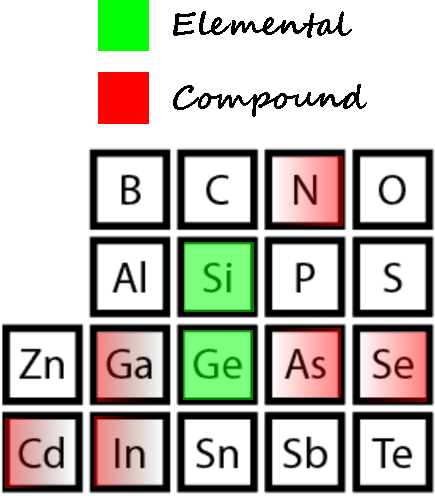
\includegraphics[width=\textwidth]{semiconductors_periodic_table}
		\end{figure}
	\end{column}
\end{columns}
%
\begin{itemize}
	\item Certain combinations of elements of Groups III and V or Groups II and VI also are semiconductors. These are called \textbf{compound semiconductors}. \ce{GaAs}, \ce{InP} are some of the well known examples.
	%
	\item 	In a semiconductor, two charge carriers, namely \textbf{electrons} and \textbf{holes}, transport current.
\end{itemize}
\end{frame}
%
\begin{frame}{Nature of bonding: Silicon crystal}
\begin{figure}
	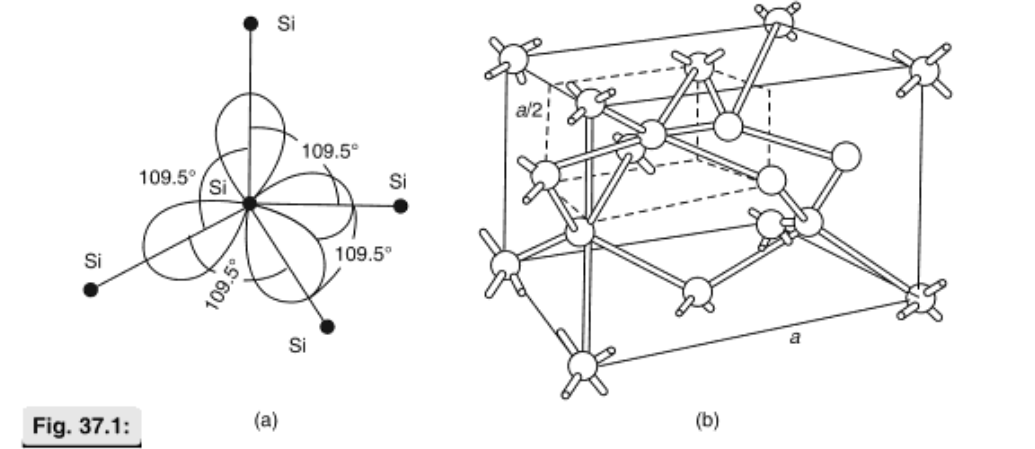
\includegraphics[width=0.6\textwidth]{semiconductors_silicon_crystal}
	\caption{(a) Tetrahedral arrangement (b) Diamond crystal structure. Taken from Avadhanulu, Chapter 37.}
\end{figure}
%
\begin{itemize}
	\item \ce{^18Si} atom has electronic configuration \ce{1s^2 2s^2 2p^6 3s^2 3p^2}.
	\item In \ce{Si} crystal, the four valence electrons undergo \textbf{hybridization} to form four \ce{sp^3} molecular orbitals. These orbitals form covalent bonds with neighbouring atoms arranged in tetrahedral arrangement. The resulting structure is the \textbf{diamond cubic crystal structure}.
\end{itemize}
\end{frame}
%
\begin{frame}{Intrinsic Semiconductor}
	\begin{itemize}
		\item Chemically pure semiconductor is called intrinsic semiconductor. \item Practically, a semiconductor is considered pure if there is less than one impurity atom per billion host atoms i.e. $< 1$~ ppb (part per billion).
		\item It has five properties
		%
		\begin{enumerate}
			\item Perfect insulator at absolute zero temperature
			\item Generation of charge carriers by thermalization
			\item Existence of energy band gap (M2U3)
			\item Conductivity is \textbf{highly} influenced by temperature
			\item Recombination of charge carriers
		\end{enumerate}
		\item For \ce{Si}, the valence electron density is of the order of \SI{e29}{\per\metre\cubed}. However, at room temperature the conduction electron density is only of the order of \SI{e18}{\per\metre\cubed}.
	\end{itemize}
	%
	\begin{guesstimate}{Valence electron density of \ce{Si}}
		The lattice constant of Si crystal is \SI{5.43}{\angstrom}.
	\end{guesstimate}
\end{frame}
%
\ifshowhidden
%
\begin{frame}{Nature of metallic bonding}
	\begin{figure}
		\centering
		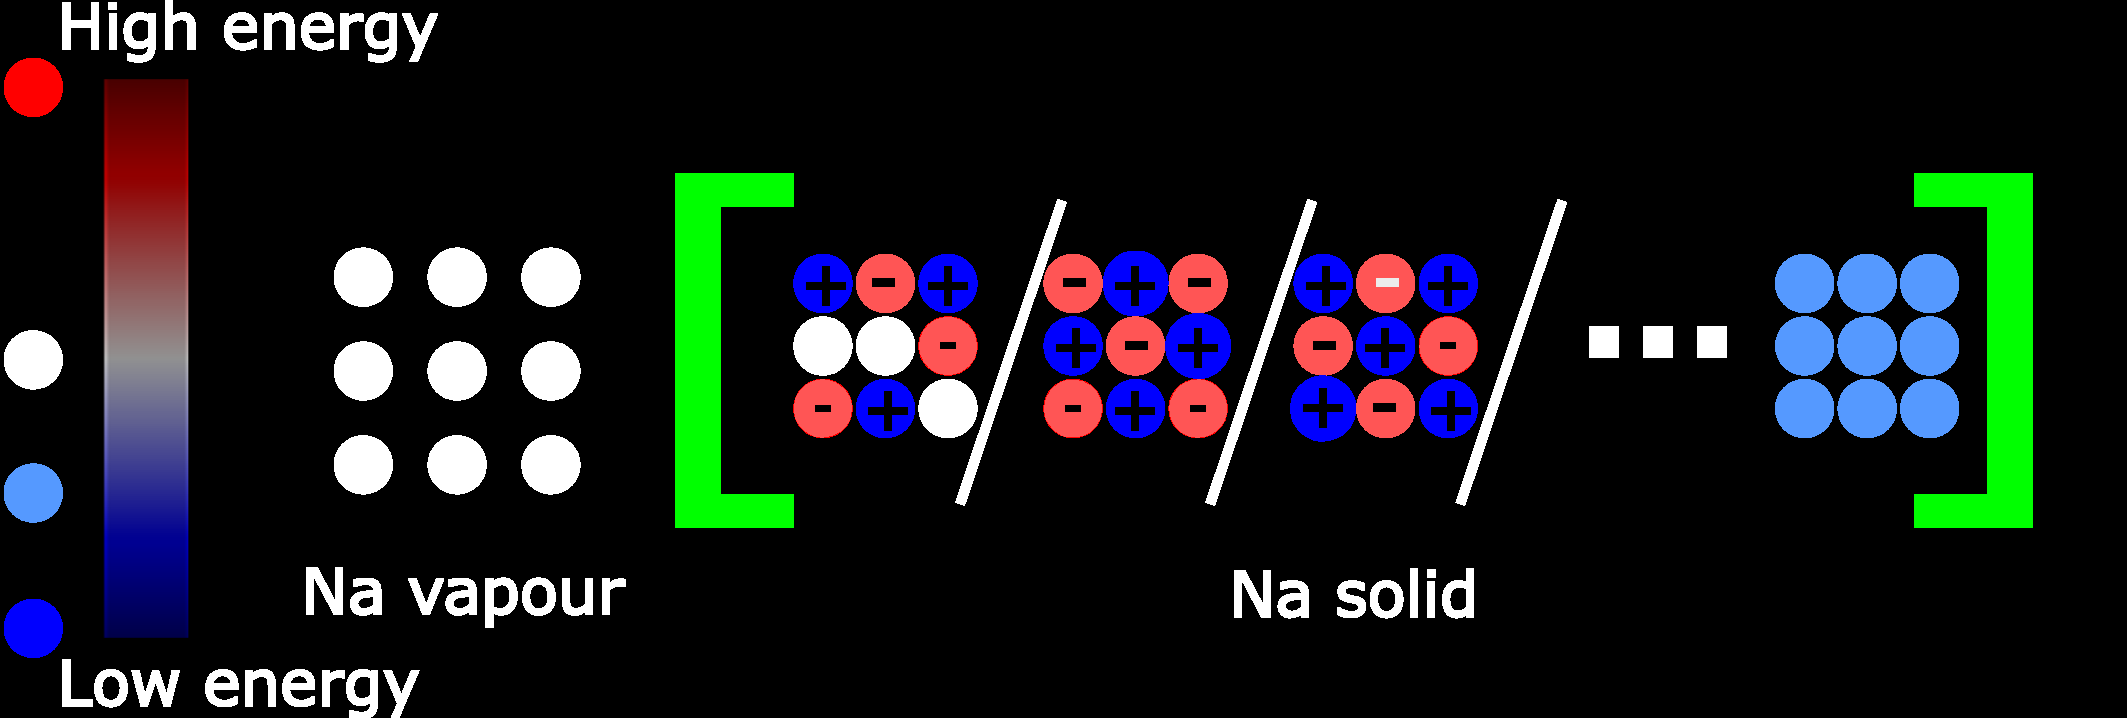
\includegraphics[width=0.8\textwidth]{semiconductors_sodium_vapour_to_solid}
	\end{figure}
	%
		\begin{itemize}
		\item When the sodium vapour condenses, the valence electrons ``hop'' onto neighbouring lattice sites. One site A looses an electron while the neighbouring site B gains an extra electron.
		\item The reduction in energy due to loss of electron at A is more than the increase in energy due to gain of electron at B. As a result, hopping is preferred resulting in \textbf{metallic bonding}.
		\item Since hopping is non directional, the metallic bond is non-directional.
		\item Thus the formation of metallic bond results in lowering of energy of \ce{Na} solid.
	\end{itemize}
\end{frame}
%
\fi
%
\begin{frame}{Nature of intrinsic semiconductor at \(T=0\) (property 1)}
	\begin{figure}
		\centering
		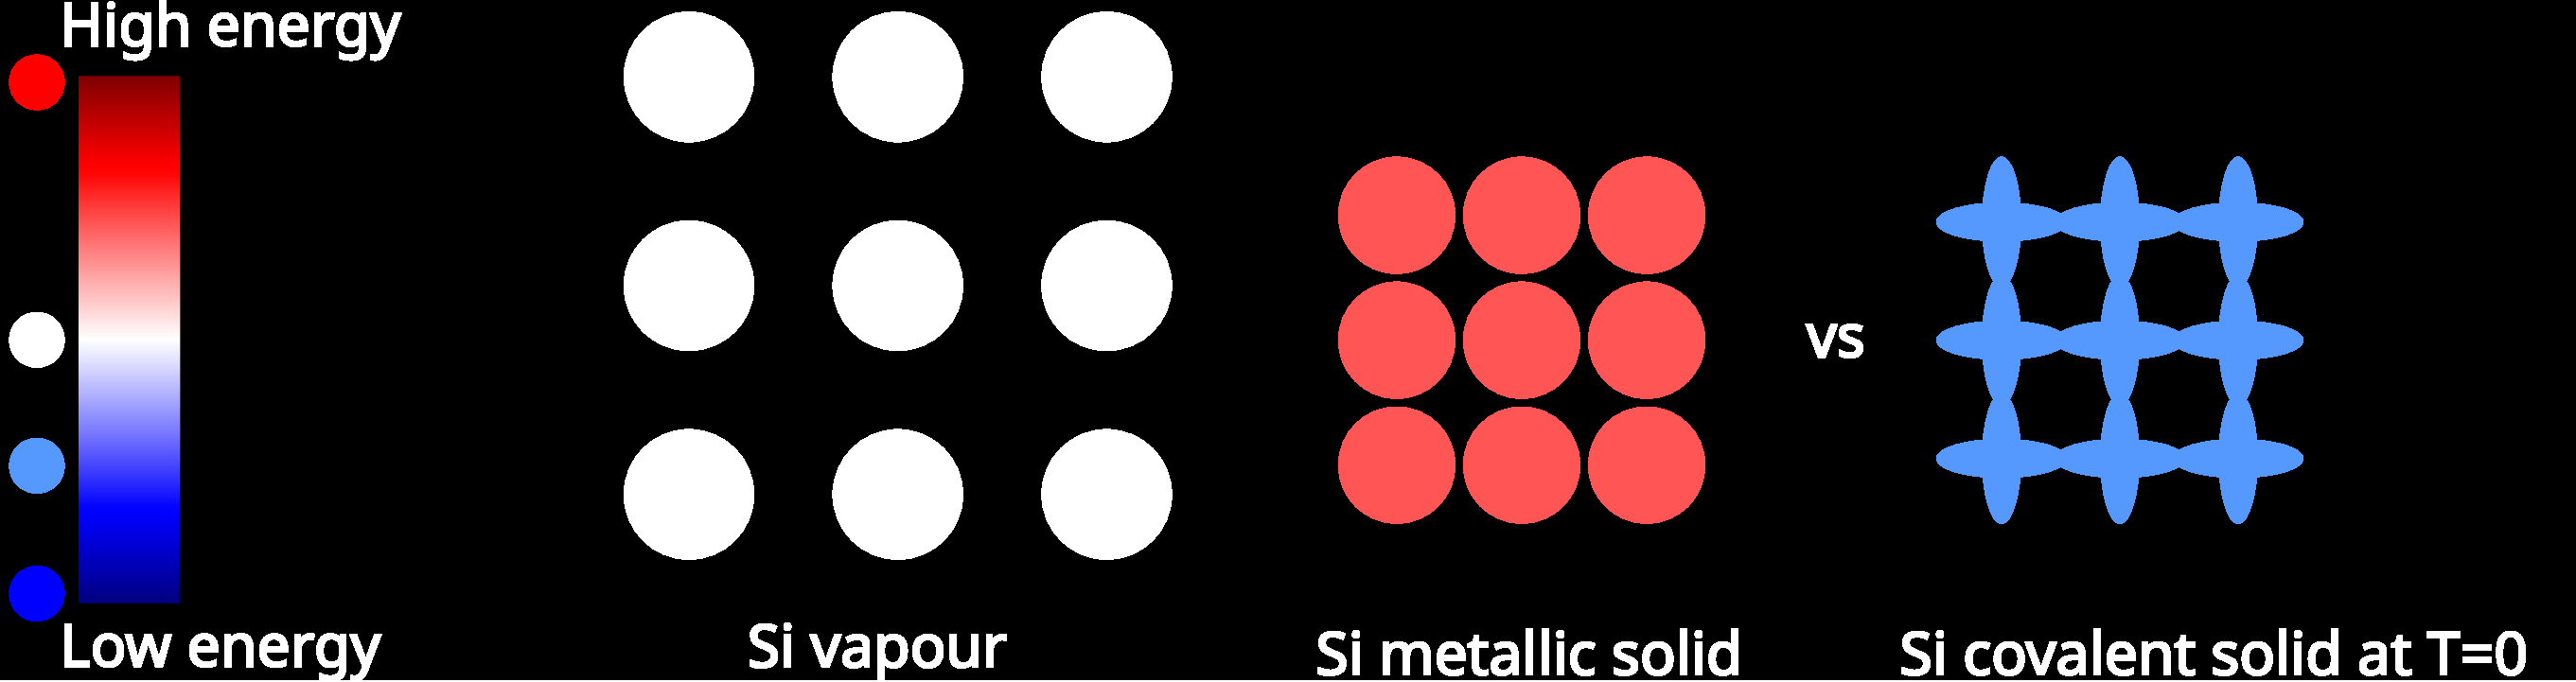
\includegraphics[width=\textwidth]{semiconductors_silicon_vapour_to_solid}
	\end{figure}
	\begin{itemize}
		\item Valence electrons are strongly attracted to the nucleus. This prevents the formation of free electron gas.
		\item Instead the valence electrons are shared between neighbouring atoms resulting in \textbf{covalent bond}.
		\item As all the valence electrons are involved in bonding, \fcolorbox{red}{white}{there are no ``free'' electrons at absolute zero temperature.}
	\end{itemize}
	%
	\begin{keyinsight}
		Intrinsic semiconductor is a perfect insulator at absolute zero!
	\end{keyinsight}
\end{frame}
%
\begin{frame}{Nature of intrinsic semiconductor at \(T\neq 0\) (property 2)}
	\begin{figure}
		\centering
		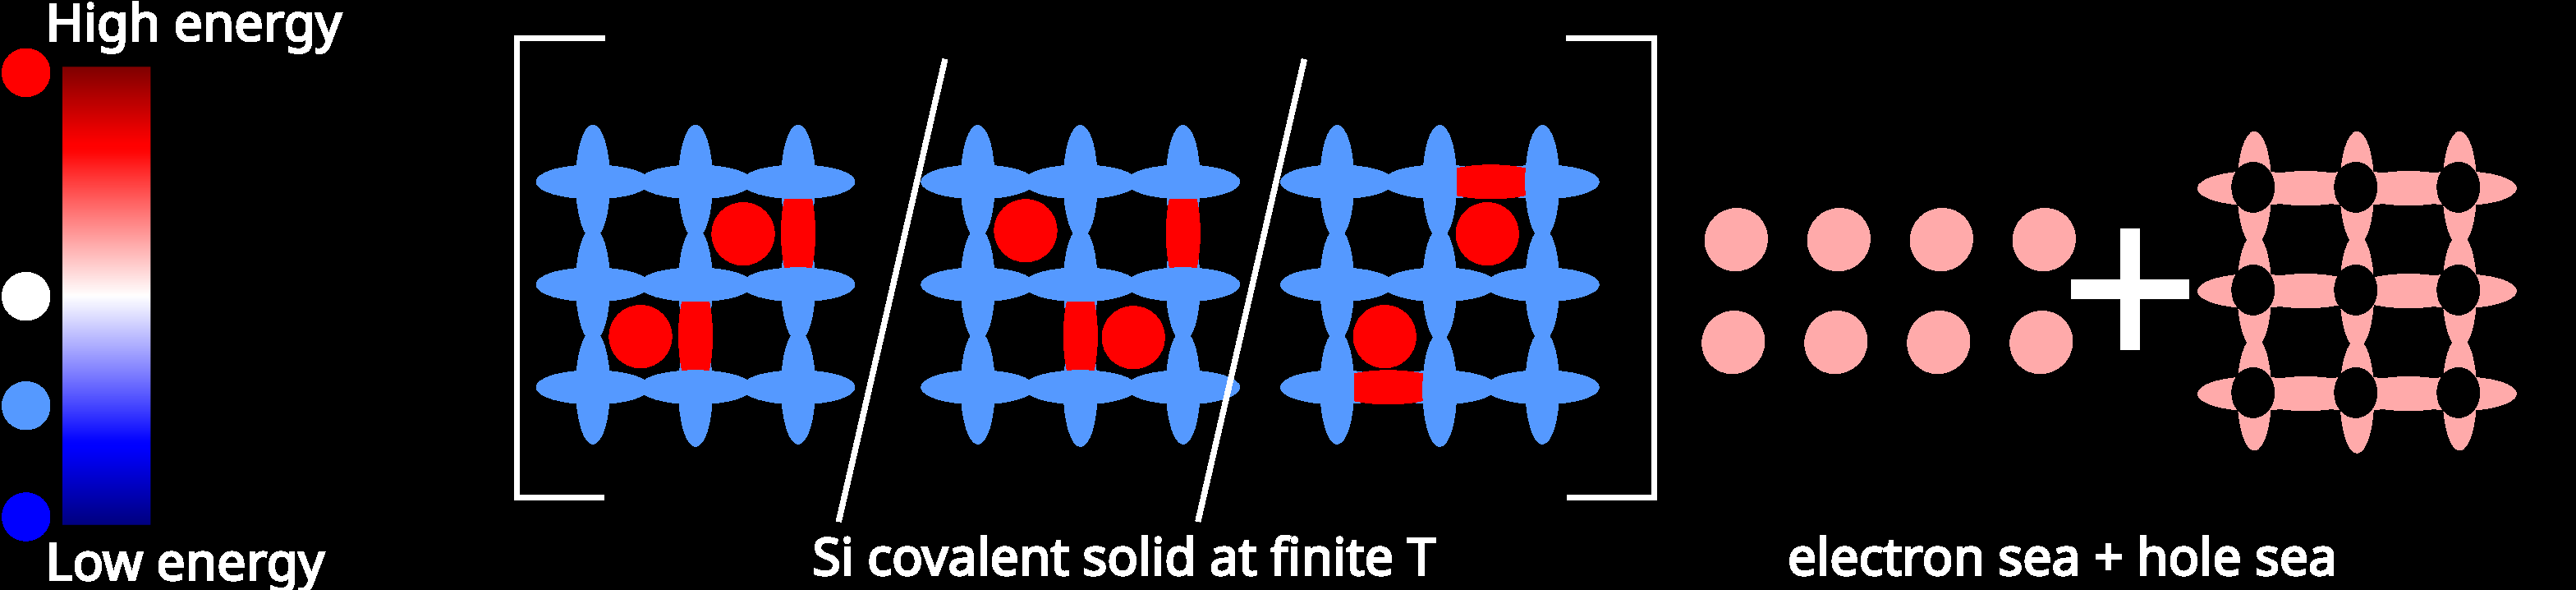
\includegraphics[width=0.8\textwidth]{semiconductors_silicon_vapour_to_solid_finite_temperature}
	\end{figure}
	%
	\vspace{-1em}
	%
	\begin{itemize}
{\small
			\item However, at finite temperature, due to thermalization, few bonds are broken, releasing the electrons to the \textbf{free electron sea}.
		\item In the process of bond breaking, the crystal lattice deficient with one electron can be considered as a new type of charge carrier. This is defined as the \textbf{hole}.
		\item The holes are released into the \textbf{free hole sea}.
		\item Every free electron is associated with a free hole. Hence they are called\textbf{ electron-hole pair}.}
	\end{itemize}
	%
	\begin{definition}
		An intrinsic semiconductor is a semiconductor crystal in which the electrical conduction arises due to \textbf{thermally excited} electrons- hole pairs.
	\end{definition}
\end{frame}
%
\begin{frame}{Nature of hole: Drift motion (property 2)}
	%
	\begin{figure}
		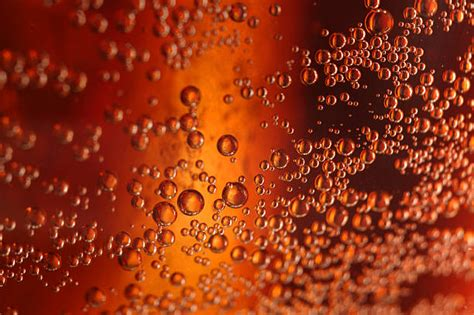
\includegraphics[height=0.3\textheight]{semiconductors_holes_analogy}
		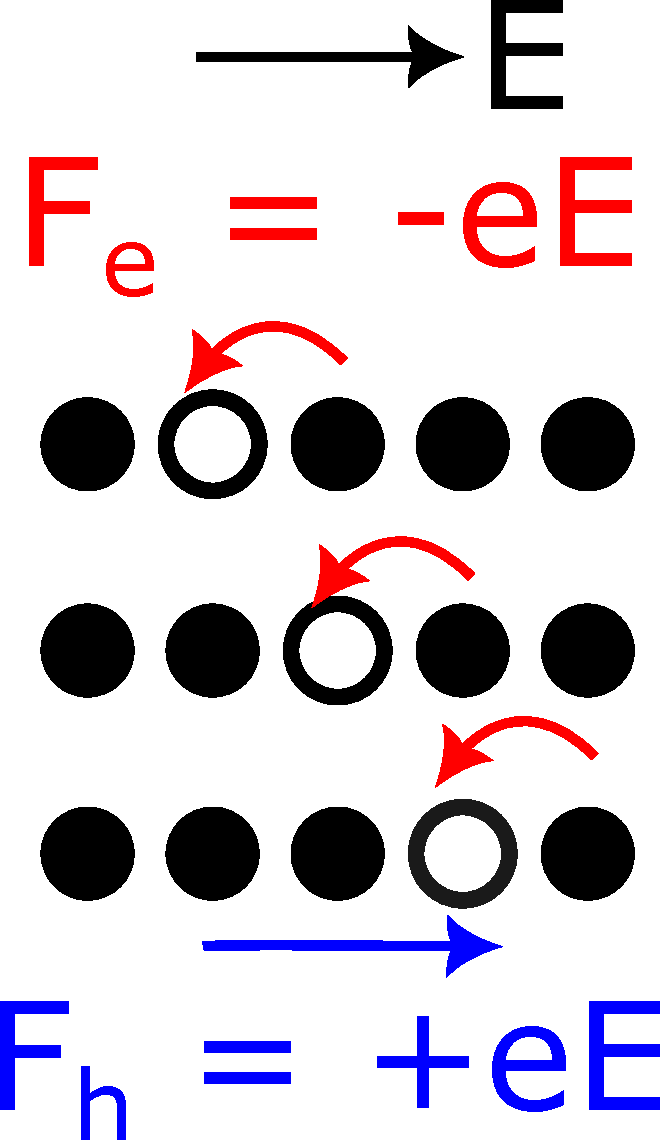
\includegraphics[height=0.3\textheight]{semiconductors_hole_drift}
		\caption{(a) Analogy for a hole: Bubbles (b) Drift motion of holes}
	\end{figure}
	%
	\vspace{-1em}
	\begin{itemize}
{\small
			\item A hole is a \textbf{quantum vacancy} that is described as an absence of electron. 
		\item Analogy is the bubbles appearing in carbonated water. The bubbles are absence of water.
		\item Under application of electric field, the bonded electrons move in the opposite direction. The hole appears to move along the electric field.}
	\end{itemize}
	%
	\begin{keyinsight}
		The motion of hole is along the electric field.
	\end{keyinsight}
	%
\end{frame}
%
\begin{frame}{Energy band gap: Chemistry view (property 3)}
	%
	\begin{figure}
		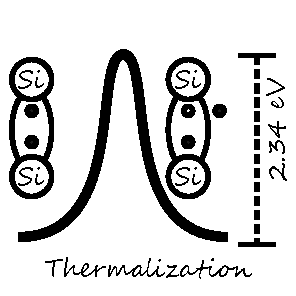
\includegraphics[height=0.25\textwidth]{semiconductors_energy_bang_gap}
	\end{figure}
	\begin{itemize}
{\small
			\item The electron of the covalent bond needs to overcome bonding strength to become free.
		\item If all the bonds are broken, then the crystal vapourizes. The energy needed to vapourize a crystal is called \textbf{cohesive energy}.
		\item The actual energy to free electron is \SI{1.12}{\electron\volt} and is called the \textbf{energy band gap} (M2U3).}
	\end{itemize}
	%
	\begin{guesstimate}{Bonding strength}
		The cohesive energy of Si crystal is \SI{450}{\kilo\joule\per\mole}. Estimate the \ce{Si-Si} bond strength.
	\end{guesstimate}
	%
\end{frame}
%
\begin{frame}{Charge carriers vs temperature (property 4)}
	\begin{figure}
		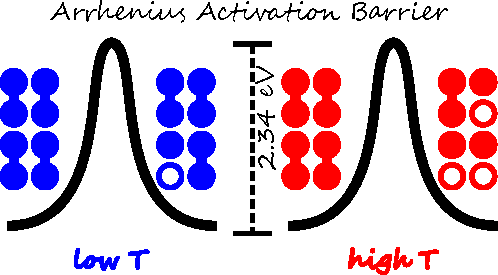
\includegraphics[height=0.25\textheight]{semiconductors_thermal_energy_vs_band_gap}
	\end{figure}
	\begin{itemize}
{\small
			\item The scale of thermal energy is given by \(k_B T\). At room temperature, the thermal energy of electron is of the order of \SI{26}{\milli\electron\volt}. \hfill [Estimate]
		\item The bond strength can be considered an \textbf{activation barrier} for the generation of electron-hole pair. This is analogous to rate of chemical reaction
		\[
		\text{covalent bond} + \text{thermal energy} \rightarrow \text{electron} + \text{hole}
		\]
		\item Electron-hole pair density increases exponentially with temperature. This follows the \textbf{Arrhenius law}.
		\[
		n \propto \exp(-\frac{1}{k_B T}) \quad p \propto \exp(-\frac{1}{k_B T})
		\]
		}
	\end{itemize}
\end{frame}
%
\begin{frame}{Conductivity vs temperature (property 4)}
	%
	\begin{figure}
		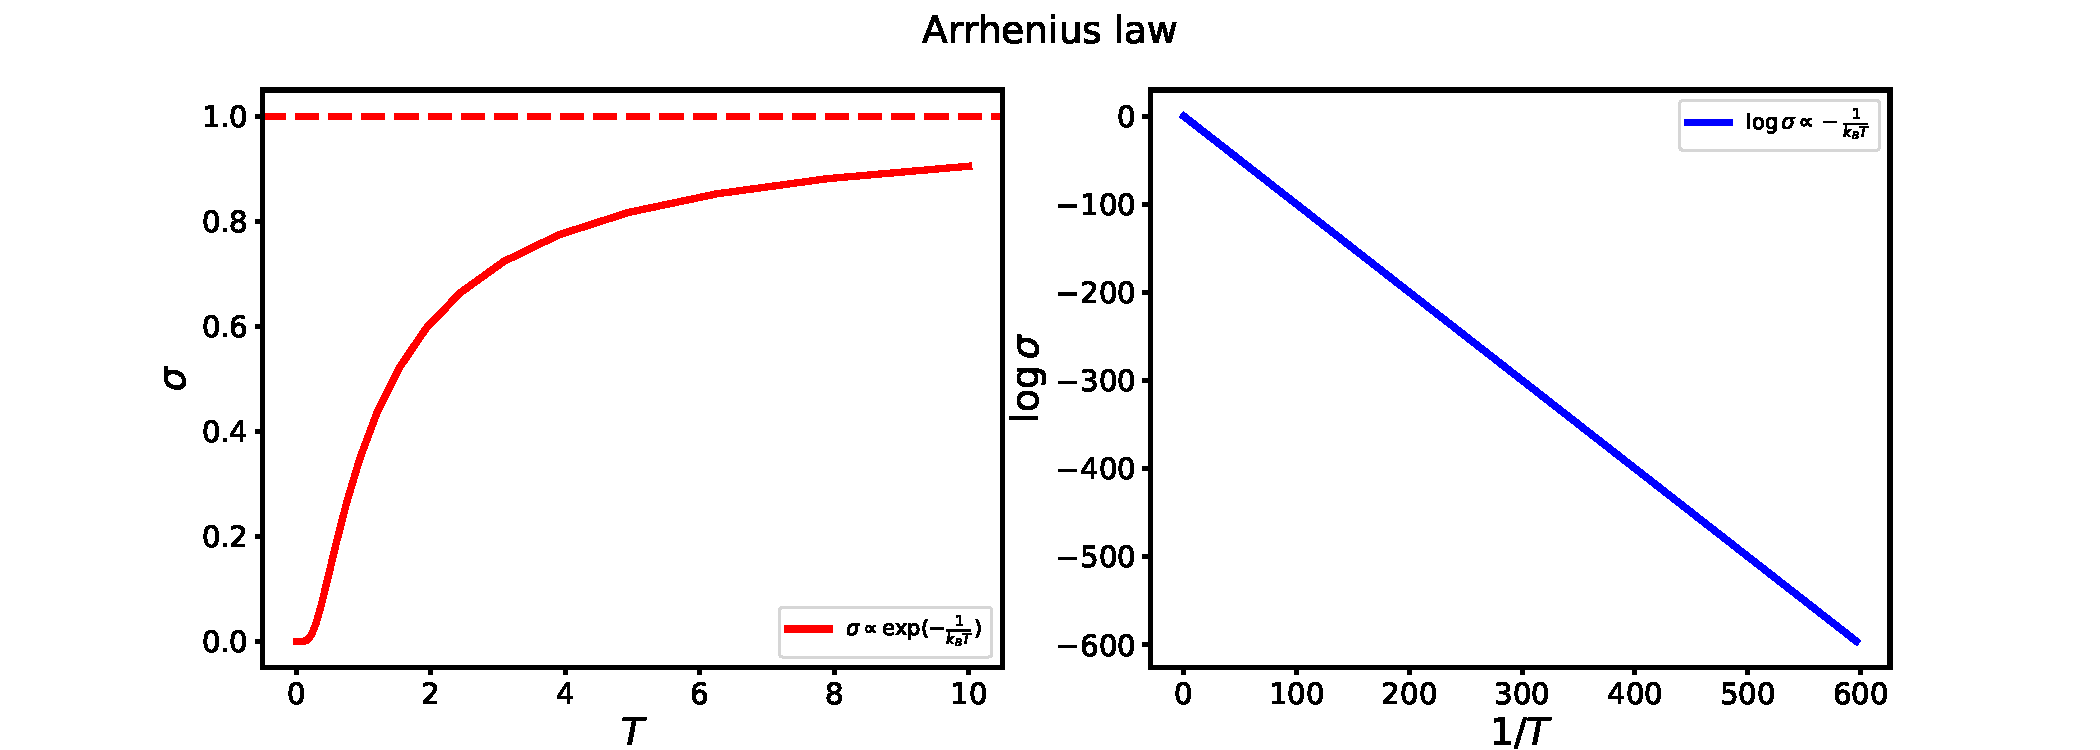
\includegraphics[height=0.4\textheight]{semiconductors_conductivity_vs_temperature}
	\end{figure}
	\begin{itemize}
		\item Since conductivity is proportional to number density, conductivity also follows Arrhenius law.
		\[
		\sigma \propto n \quad \sigma \propto p
		\]
	\end{itemize}
	\begin{keyinsight}
		Conductivity exponentially depends on temperature.
	\end{keyinsight}
\end{frame}
%
\begin{frame}{Recombination of carriers (property 5)}

		\begin{itemize}
			{\footnotesize
		\item We have seen thermal energy to generate electron-hole pairs. This is an example of \textbf{equilibrium} generation
		\item Light can also be used to generate electron-hole pairs. 
		\[
		\text{covalent bond} + \text{light} \rightarrow \text{electron} + \text{hole}
		\]
		However, this is a \textbf{non-equilibrium} generation process.
		\item The reverse process where the electron-hole pairs combine to become part of the covalent lattice is called \textbf{recombination}.
		\[
		\text{electron} + \text{hole} \rightarrow \text{covalent bond} +  \text{light} / \text{lattice vibration}
		\]
		The additional energy is released either as light (\textbf{photon}) or lattice vibration (\textbf{phonon}).
		\item The generation-recombination of charge carriers is a \textbf{dynamic} two way process.
	}
	\end{itemize}

	%
	\begin{keyinsight}
		For analysis, a semiconductor is a collection of electron, holes, photons and phonons and the interaction between them.
	\end{keyinsight}
\end{frame}
%
\begin{frame}{Applications of intrinsic semiconductor: Switch}
\begin{columns}
	\begin{column}[t]{0.6\textwidth}
			\begin{figure}
		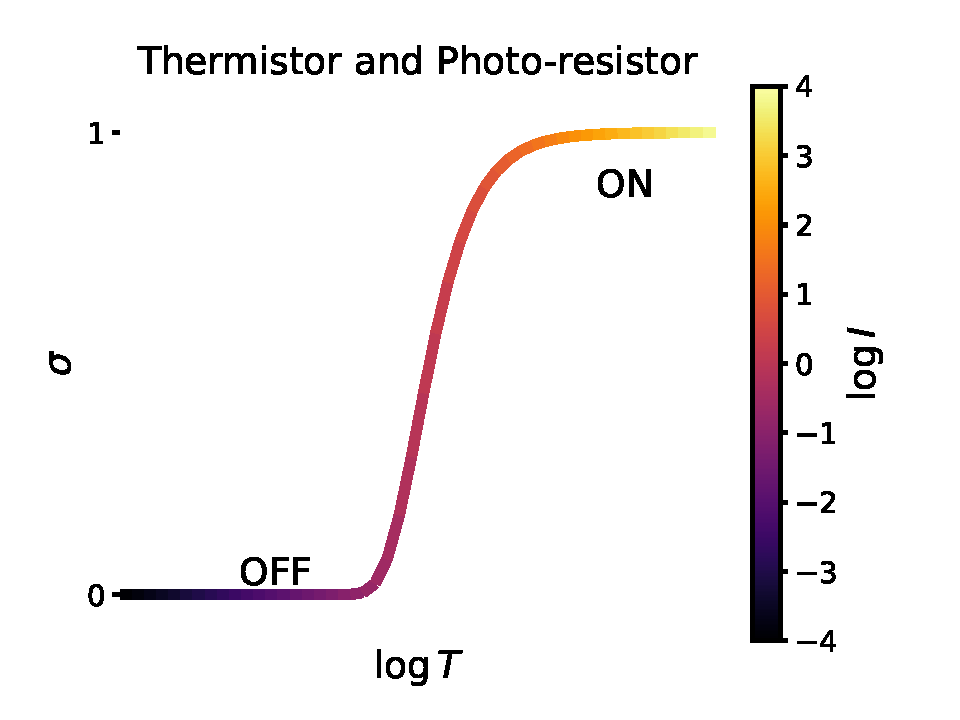
\includegraphics[width=\textwidth]{semiconductors_LDR}\\
		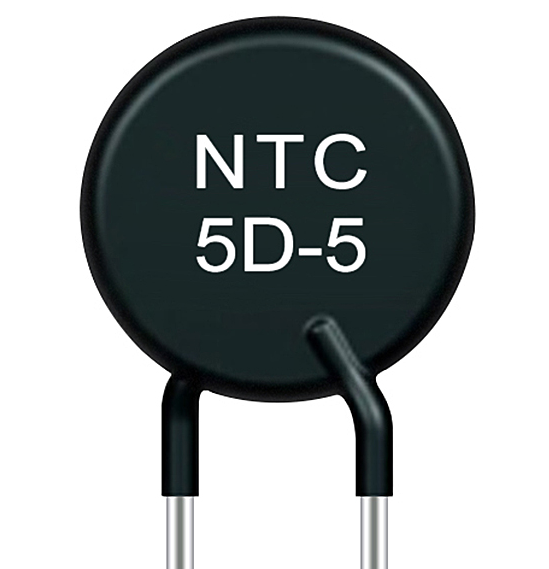
\includegraphics[width=0.25\textwidth]{semiconductors_thermistor_component}
		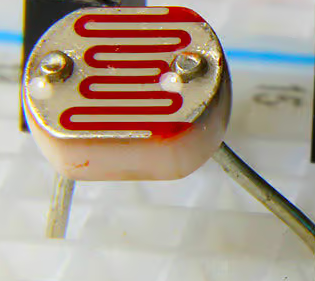
\includegraphics[width=0.25\textwidth]{semiconductors_photoresistor_component}
	\end{figure}
	\end{column}
	%
	\begin{column}[t]{0.38\textwidth}
{\small
			\begin{itemize}
			\item Thermistor (Temperature dependent resistor). Generation of carriers by temperature.
			\item Photo-resistor: (Light Dependent Resistor (LDR)). Generation of carriers by light.
		\end{itemize}
		%
		\begin{table}
			\centering
			\begin{tabular}{l l}
				\toprule
				App	&	Material	\\
				\midrule
				Thermistor	&	\ce{Fe3O4}\\
				Photoresistor	&	\ce{CdSe}\\
				\bottomrule
			\end{tabular}
		\end{table}}
	\end{column}
\end{columns}
%
\end{frame}
%
\begin{frame}{Application of thermistor: Smartphone}
	%
		\begin{figure}
		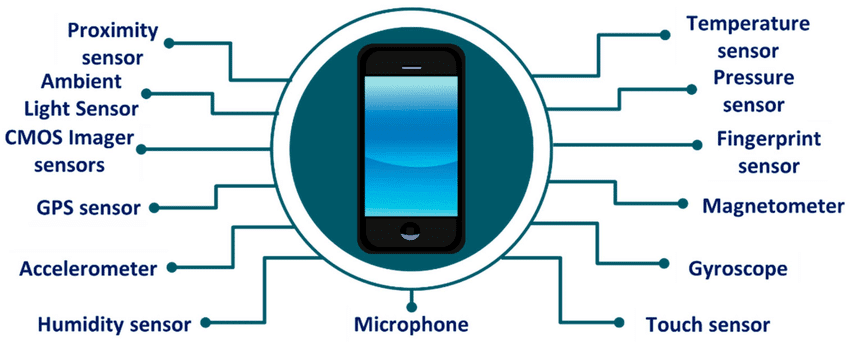
\includegraphics[width=0.8\textwidth]{qm_sensors_in_smartphone}
		\caption{Image taken from Techbii.com. \href{https://techbii.com/10-most-important-sensors-mobile-phones-uses/}{Click here for link}}
	\end{figure}
	%
	\begin{itemize}
		\item temperature sensor to monitor chip and battery health
	\end{itemize}
\end{frame}
%
\begin{frame}{Extrinsic semiconductor}
	\begin{itemize}
		\item The electrical properties of intrinsic semiconductor can be altered by adding impurities.
		\item The technique of adding controlled impurity is called \textbf{doping} and the impurity added is called \textbf{dopant}.
		\item Doped semiconductor is called \textbf{extrinsic} semiconductor.
		\item Dopant atom substitutes the position of parent atom. The dopants are of two types -- donor and acceptor.

		\item For \ce{Si}, donors are \ce{P}, \ce{As}, etc and acceptors are \ce{B}, \ce{Al}, etc.
		\item For \ce{P} as a donor dopant, four valence electrons contribute to covalent bonding. The fifth electron is loosely bound to the phosphorus atom
		\item For \ce{B} as an acceptor dopant, three valence electrons contribute to covalent bonding.
	\end{itemize}
	%
	\begin{guesstimate}{Dopant concentration}
		\ce{P} doping is 1 ppm. \hfill \(n_{valence} \sim \) \SI{2e23}{\per\centi\metre\cubed}
	\end{guesstimate}
\end{frame}
%
\begin{frame}{Ionization energy of dopants}
	%
	\begin{definition}
		The energy required to ionize a dopant atom is called ionization energy.
	\end{definition}
	%
	{\footnotesize
	\begin{itemize}
		\item Lattice vibrations (phonons) supply the ionization energy (I.E.)
		\item For \ce{P} as donor dopant,
		\[
		\ce{P + I.E. -> P^+ + e}
		\]
		\item Similarly, for \ce{B} as acceptor dopant,
		\[
		\ce{B + I.E. -> B^- + h}
		\]
		\item If thermal energy (\(E_{th}\)) is greater than I.E. \(E_{ion}\), then ions are completely ionized. This is called \textbf{complete} ionization.
		\item For \(E_{th} \ll E_{ion}\), there is no ionization. This is called \textbf{freeze out}.
		\item \textbf{Partial} ionization occurs when \(E_{th} \lesssim E_{ion}\) 
		\item In \ce{Si}, \(E_{ion} \, \sim \) \SI{25}{\milli\electron\volt} and  \(E_{th} \, \sim\)\SI{25}{\milli\electron\volt} at room temperature. Thus, the ions are \textbf{completely ionized}.
	\end{itemize}}
\end{frame}
	%\fi
	%
	\section{Electrical conductivity of semiconductors}
	%
	%\ifshowhidden
	%
\againframe{plan}
%
\begin{frame}{Conductivity}
	In a semiconductor, there are two types of charge carriers -- electrons and holes. Each carrier is associated with corresponding mobility. Thus, the mobility of electrons is \(\mu_e\) and that of holes is \(\mu_h\).
	\\
	From the classical free electron theory, the conductivity in terms of mobility and charge density is given by
	\[
	\sigma = n e \mu
	\]
	In semiconductors, there are\textbf{ two channels} for conduction. Thus, the conductivity adds up and is given by
	\[
	\sigma = n e \mu_e + p e \mu_h
	\]
	\begin{keyinsight}
		Both electrons and holes contribute to conductivity 
	\end{keyinsight}
\end{frame}
%
\begin{frame}{Drift motion of electrons and holes}
	%
	\begin{columns}
		\begin{column}{0.6\textwidth}
			\begin{itemize}
				\item Under electric field, electron and hole drift motion is \textbf{anti-parallel}.
				\[
				\vb{F}_e = - q_e \vb{E}, \qquad \vb{F}_h = + q_h \vb{E}.
				\]
			\end{itemize}
		\end{column}
		%
		\begin{column}{0.38\textwidth}
			\begin{figure}
				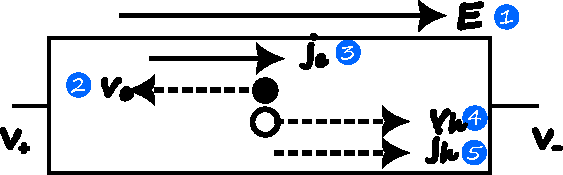
\includegraphics[width=\textwidth]{semiconductors_drift_current}
			\end{figure}
		\end{column}
	\end{columns}
	%
	\begin{itemize}
		\item The sign of their charges are opposite.
		\item Electron and hole drift current direction is  \textbf{parallel}.
		\item The total drift current density is given by \hfill \(\vb{j}_\mathrm{drift} = \vb{j}_e + \vb{j}_h\).
		\item Drift current is proportional to electric field. \hfill
		\(
		\vb{j}_\mathrm{drift} = \sigma_e \vb{E} + \sigma_h \vb{E}
		\)
		\item Conductivity is written in terms of carrier density and mobility
		\[
		\sigma_e = n e \mu_e, \qquad \sigma_h = p e \mu_h,
		\]
		\item The drift conductivity is given by
		\[
		\sigma_\mathrm{drift} =  n e \mu_e +  p e \mu_h
		\]
	\end{itemize}
\end{frame}
\begin{frame}{Intrinsic semiconductor}
\begin{columns}
	\begin{column}{0.6\textwidth}
			For the intrinsic case, the number density of electrons equals the number density of holes
	\[
	n = p = n_i
	\]
	Thus, the conductivity is given by
	\[
	\sigma = n_i e \big(\mu_e + \mu_h\big)
	\]
	\end{column}
	%
	\begin{column}{0.38\textwidth}
\begin{small}
			\begin{figure}
			\begin{tabular}[t]{l l}
				\toprule
				Carrier density	&	\si{\per\centi\metre\cubed}	\\
				\midrule
				\(n_\mathrm{i-Si}\)	&	\num{e10}	\\
				\(n_\mathrm{Cu}\)&	\num{e22}	\\
				\bottomrule
			\end{tabular}
			%
			\\
			%
			\begin{tabular}[t]{l l}
				\toprule
				Mobility	&	\si{\centi\meter\squared\per\volt\per\second}	\\
				\midrule
				\(\mu_e\) [Si]	&	1400	\\
				\(\mu_h\) [Si]	&	500	\\
				\(\mu\) [Cu]	&	40	\\
				\bottomrule
			\end{tabular}
		%	\caption{At \SI{300}{\kelvin}.}
		\end{figure}
\end{small}
	\end{column}
\end{columns}
%
\begin{guesstimate}{Conductivity of intrinsic \ce{Si}}
	Compare it with conductivity of copper.
\end{guesstimate}
%
\begin{keyinsight}
	Though the carrier mobility in metals is less than in semiconductors, \textbf{very much higher} carrier density leads to higher metallic conductivity.   
\end{keyinsight}
\end{frame}
%
\begin{frame}{Extrinsic semiconductor}
	\begin{columns}
		\begin{column}{0.48\textwidth}
			\begin{itemize}
				\item n-type: Electrons are \textbf{majority} charge carriers
					\[
					n \gg p, \quad \text{so that} \quad ne\mu_e \gg pe\mu_h 
					\]
					\[
					\therefore	\sigma \simeq ne \mu_e
					\]
			\end{itemize}
			%
		\end{column}
		%
		\begin{column}{0.48\textwidth}
			\begin{itemize}
				\item p-type: Holes are \textbf{majority} charge carriers
					\[
					p \gg n, \quad \text{so that} \quad pe\mu_h \gg ne\mu_e   
					\]
					\[
					\therefore \sigma \simeq pe \mu_h
					\]
			\end{itemize}
		\end{column}
		%
	\end{columns}
	%
	\begin{small}
		\begin{table}
			\begin{tabular}{l l l}
				\toprule
				Material	&	\(n\) (in \si{\per\centi\metre\cubed})	&	\(\sigma\) (in \si{\siemens\per\metre}	)\\
				\midrule
				\ce{i-Si}	&	\num{e10}	&	\num{e-4}	\\
				\SI{1}{\ppm} \ce{n-Si}	&	\num{e16}	&	\num{e+2}	\\
				\bottomrule
			\end{tabular}
		\end{table}
		
	\end{small}
	%
	\begin{guesstimate}{Conductivity of extrinsic n-type Si}
		\ce{P} doping is \SI{5e16}{\per\centi\metre\cubed}. Compare it with conductivity of intrinsic-\ce{Si}.
	\end{guesstimate}
	%
	\begin{keyinsight}
		Doping of the order of \SI{1}{\ppm} increases conductivity of silicon by six orders of magnitude.
	\end{keyinsight}
\end{frame}
	%\fi
	%
	\section{Hall effect}
	%
	%\ifshowhidden
	%
\againframe{plan}
%
\begin{frame}{Hall effect}
\begin{columns}
	\begin{column}[t]{0.8\textwidth}
		\begin{itemize}
	\item	In the presence of magnetic field acting perpendicular to the flow of electrons, the electrons experience a Lorentz force that deviates their path in the transverse direction. Accumulation of electrons along the edges leads to generation of voltage. This is called \textbf{Hall effect}.
\end{itemize}
	\end{column}
	%
	\begin{column}[t]{0.18\textwidth}
		\begin{figure}
			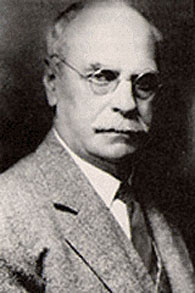
\includegraphics[width=\textwidth]{Edwin_Herbert_Hall__1855_1938}
			{\centering\footnotesize E. Hall }
		\end{figure}
	\end{column}
\end{columns}
%
\begin{itemize}
	\item Hall effect is prominent in two dimensional geometry and can be considered the advent of research on thin films.
	\item It was discovered before the discovery of electron!
	\item In the context of semiconductors, Hall effect has contribution from holes, in addition to electrons. It also helps determine
	\begin{itemize}
		\item the type of semiconductor (n or p),
		\item the majority carrier concentration, and
		\item the majority carrier mobility.
	\end{itemize}
\end{itemize}
\end{frame}
%
\begin{frame}{Hall effect: Lorentz force}
\begin{columns}
	\begin{column}{0.8\textwidth}
		\begin{itemize}
		\item In the presence of electric field \(\vb{E}\) and magnetic field \(\vb{B}\), the electron experiences a force given by
		\begin{align*}
			 \vb{F}_\mathrm{Lorentz} &= \vb{F}_\mathrm{elec} +  \vb{F}_\mathrm{mag} \\
			 &= -e \vb{E} -e \vb{v} \times \vb{B}
		\end{align*}
	\end{itemize}
	\end{column}
	%
	\begin{column}{0.18\textwidth}
		\begin{figure}
			\begin{overpic}[width=\textwidth]{Hendrik_Lorentz_1853_1928}
				% Overlay image on top
				\put(0,0){\includegraphics[width=0.4\textwidth]{Alfred_Nobel_1833_1896}}
			\end{overpic}
			\\
			{\centering\footnotesize H. Lorentz }
		\end{figure}
	\end{column}
\end{columns}
\end{frame}
%
\begin{frame}{Hall effect: experiment}
	\begin{figure}
		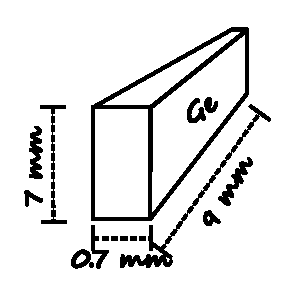
\includegraphics[width=0.32\textwidth]{hall_effect_circuit diagram_1}
		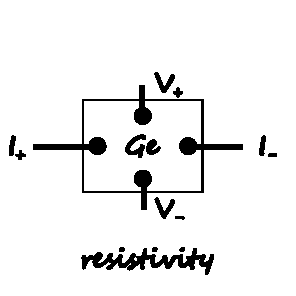
\includegraphics[width=0.32\textwidth]{hall_effect_circuit diagram_2}
		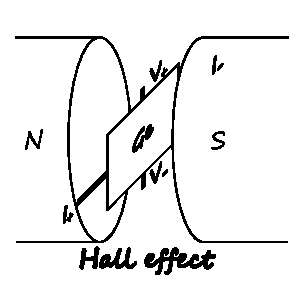
\includegraphics[width=0.32\textwidth]{hall_effect_circuit diagram_3}
	\end{figure}
	%
	\begin{itemize}
		\item The aim is to find the charge carrier type of Germanium crystal of dimensions \SI{9}{\milli\metre} x \SI{7}{\milli\metre} x \SI{0.7}{\milli\metre}.
		\item The resistivity is measured in the \textbf{four-probe geometry}. 
		\item Current is applied along \(x\) direction.
		\item Magnetic field of \SI{0.1}{\tesla} is applied along \(z\) direction. \hfill [\SI{1}{\tesla}=\SI{e4}{\gauss}]
		\item The Hall voltage is measured along \(y\) direction. 
	\end{itemize}
\end{frame}
%
\begin{frame}{Hall effect in p-type semiconductor}
\begin{columns}
	\begin{column}{0.4\textwidth}
		\begin{figure}
		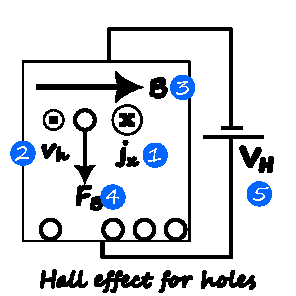
\includegraphics[width=\textwidth]{hall_effect_circuit diagram_5}
	\end{figure}
	\end{column}
	%
	\begin{column}{0.58\textwidth}
			\begin{enumerate}
			\item Current along \(x\).
			\item Electron drift along \(x\).
			\item Magnetic field along \(z\).
			\item Magnetic force along \(-y\).
			\item The buildup of holes \textbf{induces} an electric field in the \(+y\) direction.
			\item The corresponding voltage across the width is positive.
		\end{enumerate}
	\end{column}
\end{columns}
%
\end{frame}
%
\begin{frame}{Hall effect in n-type semiconductor}
	\begin{columns}
		\begin{column}{0.4\textwidth}
			\begin{figure}
				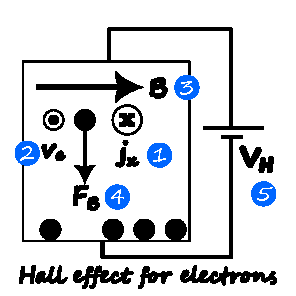
\includegraphics[width=\textwidth]{hall_effect_circuit diagram_4}
			\end{figure}
		\end{column}
		%
		\begin{column}{0.58\textwidth}
			\begin{enumerate}
				\item Current along \(x\).
				\item Electron drift along \(-x\).
				\item Magnetic field along \(z\).
				\item Magnetic force along \(-y\).
				\item The buildup of electrons \textbf{induces} an electric field in the \(-y\) direction.
				\item The corresponding voltage across the width is negative.
			\end{enumerate}
		\end{column}
	\end{columns}
	%
\end{frame}
%
\begin{frame}{Hall field and Hall voltage}
	\begin{itemize}
		\item In the steady state, the magnetic field force is balanced by the induced electric field
		\[
		\vb{F} = q(\vb{E} + \vb{v} \times \vb{B}) = q(E_y - v_x B_z) = 0
		\]
		\item The induced electric field, called the \textbf{Hall field} is given by
		\begin{center}
			\framebox{$
				E_y =  v_x B_z.
			$}
		\end{center}
		\item The Hall field produces a voltage across the semiconductor, which is called the \textbf{Hall voltage} given by
		\[
		V_H = E_H w
		\]
		where \(w\) is the width of the semiconductor.
		\item The Hall voltage is positive for p-type and negative for n-type semiconductor.
	\end{itemize}
\end{frame}
%
\begin{frame}{Hall coefficient}
	\begin{definition}
		Hall coefficient \(R_H\) is defined as the Hall field per unit current density per unit magnetic field.
	\end{definition}
	%
	\begin{itemize}
		\item \(R_H\) is given by
		\[
			R_H := \frac{E_H}{j_x B_z} = \frac{v}{j_x}
		\]
		\item \(E_H\) is positive for holes and negative for electrons.
		\item However, the current density \(j\) is related to the drift velocity \(v\) by
		\[
		j = n e v \qquad [ j = p e v \quad \text{for holes}]
		\]
		\item Therefore,
		%
\begin{center}
			\framebox{$
			R_H (\mathrm{electron}) = -\frac{1}{ne} , \qquad  R_H (\mathrm{hole}) = +\frac{1}{pe}
			$}
\end{center}

	\end{itemize}
\end{frame}
%
%
\begin{frame}{Charge carrier properties}
	\begin{itemize}
		\item Semiconductor type: The sign of Hall voltage determines the type of majority carrier in a semiconductor
		\item Majority carrier density: The Hall coefficient gives the majority carrier density as
		\begin{center}
					\framebox{
				$
				n = \frac{1}{R_H e}
				$
				}
		\end{center}
		\item Majority carrier mobility: If the conductivity of the semiconductor \(\sigma\) is measured in the absence of magnetic field, then the mobility of majority carriers is given by
		\begin{center}
			\framebox{
				$			
				\mu = \frac{\sigma}{ne}
				$
				}
		\end{center}
	\end{itemize}
\end{frame}
%
\begin{frame}{Test your Understanding}
%
	\begin{problem}
		\begin{figure}
	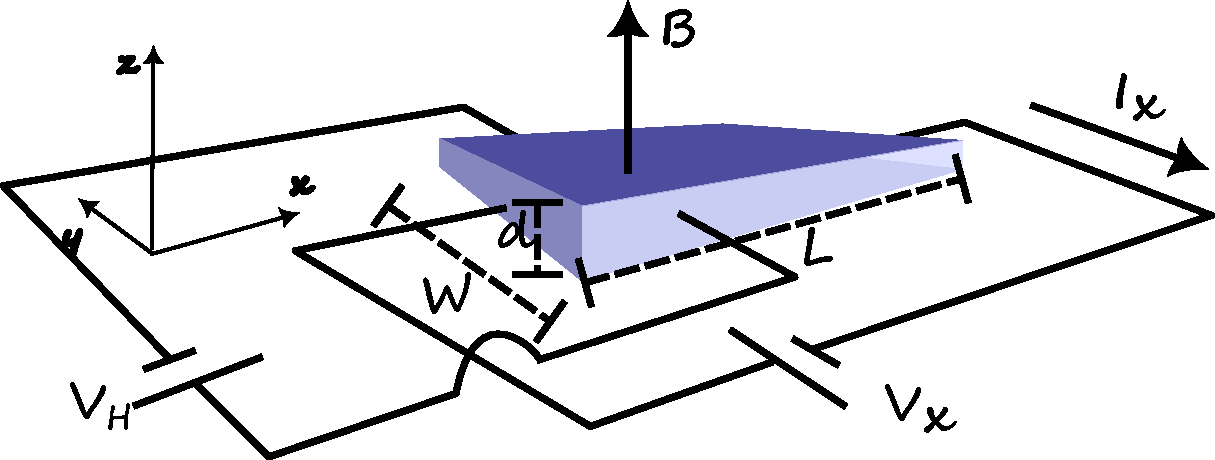
\includegraphics[width=\textwidth]{hall_effect_test_ur_understanding}
	%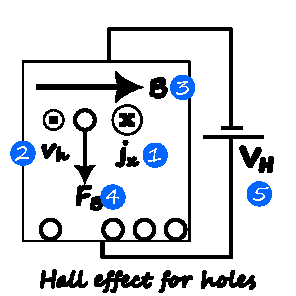
\includegraphics[width=0.3\textwidth]{hall_effect_circuit diagram_5}
\end{figure}
		%
		Determine the majority carrier type, concentration and mobility. \(L = \SI{e-1}{\centi\metre}\), \(W = \SI{e-2}{\centi\metre}\),  \(d = \SI{e-3}{\centi\metre}\). \(I_x = \SI{1}{\milli\ampere}\), \(V_x = \SI{12.5}{\volt}\), \(B = \SI{500}{\gauss}\), \(V_H = \SI{-6.25}{\milli\volt}\).
	\end{problem}
\end{frame}
\begin{frame}{Applications of Hall effect}
	\begin{itemize}
		\item Magnetic sensor: Hall voltage is directly proportional to Magnetic field 
		\begin{itemize}
			\item Gaussmeter
			\item Compass sensor in smartphones
			\item Current measurement without direct contact
		\end{itemize} 
		%
		\begin{figure}
			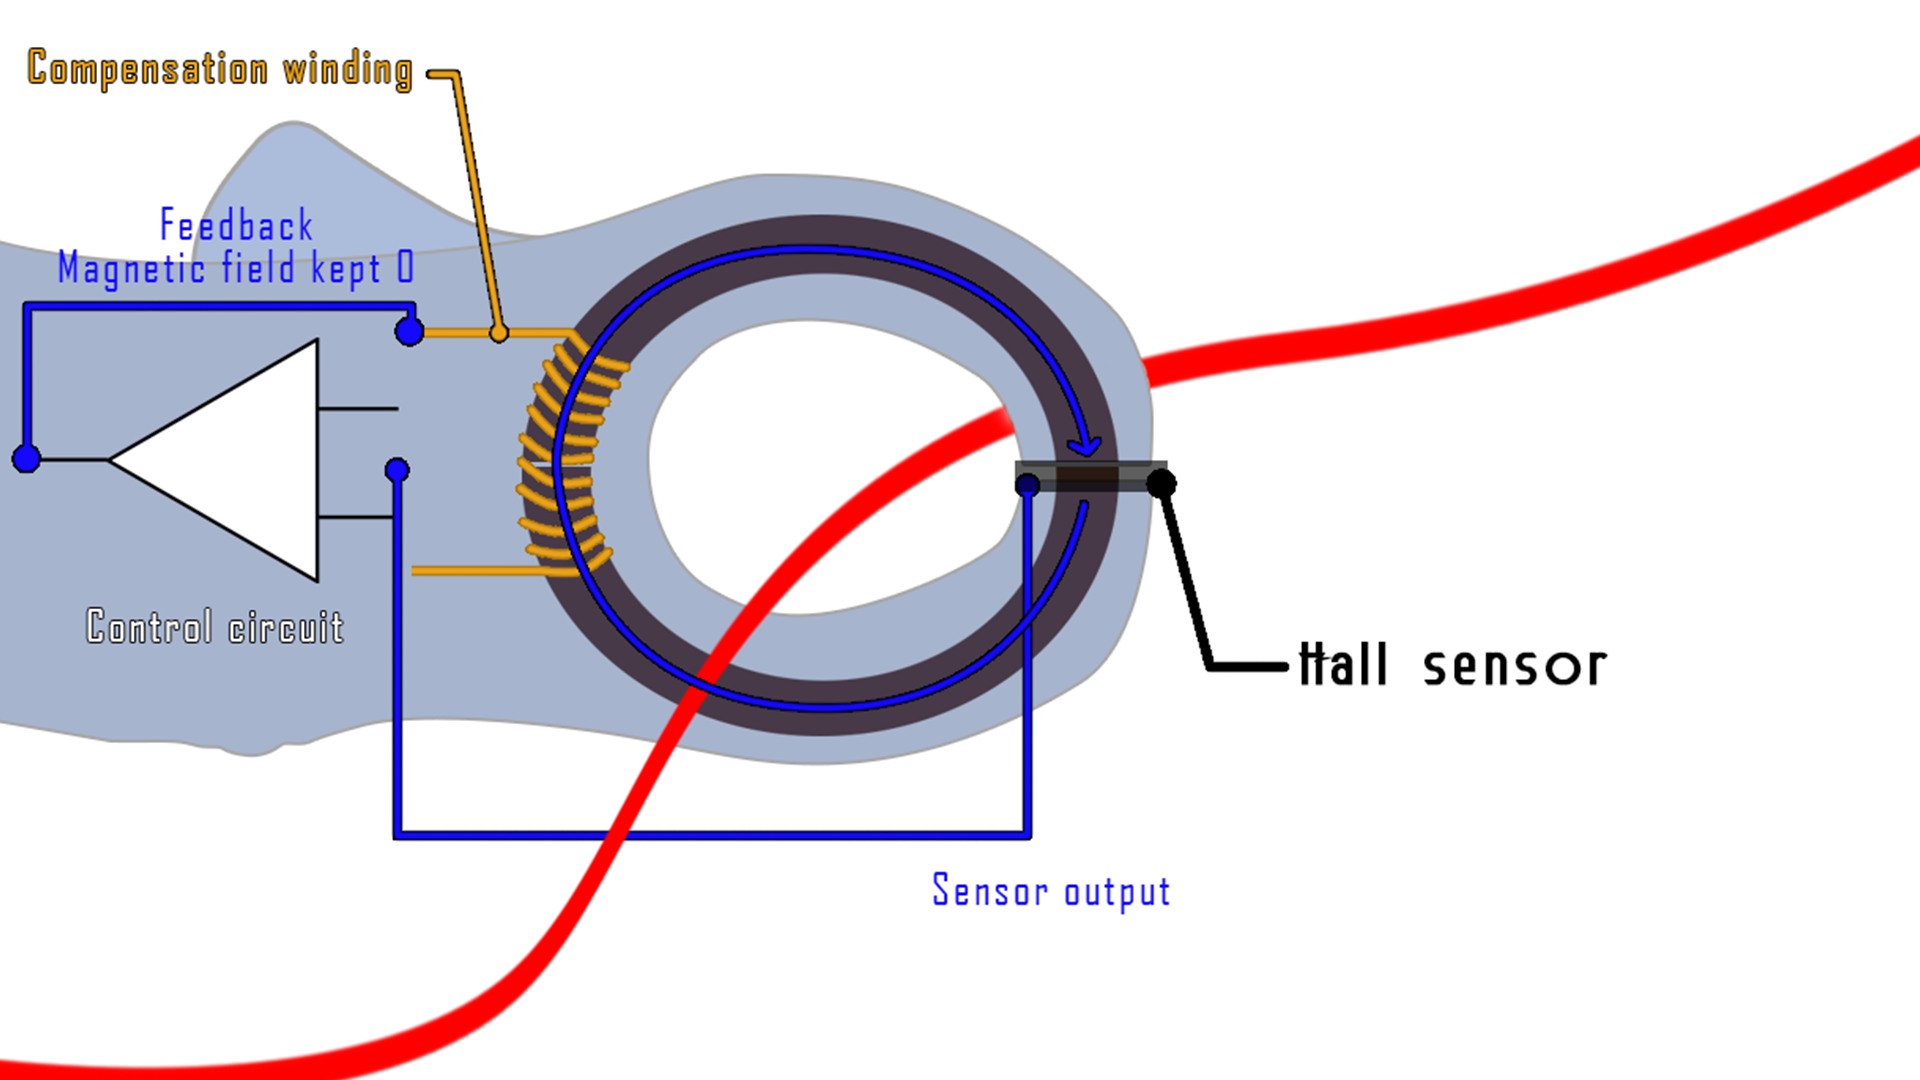
\includegraphics[width=0.45\textwidth]{hall_effect_sensor_current}
			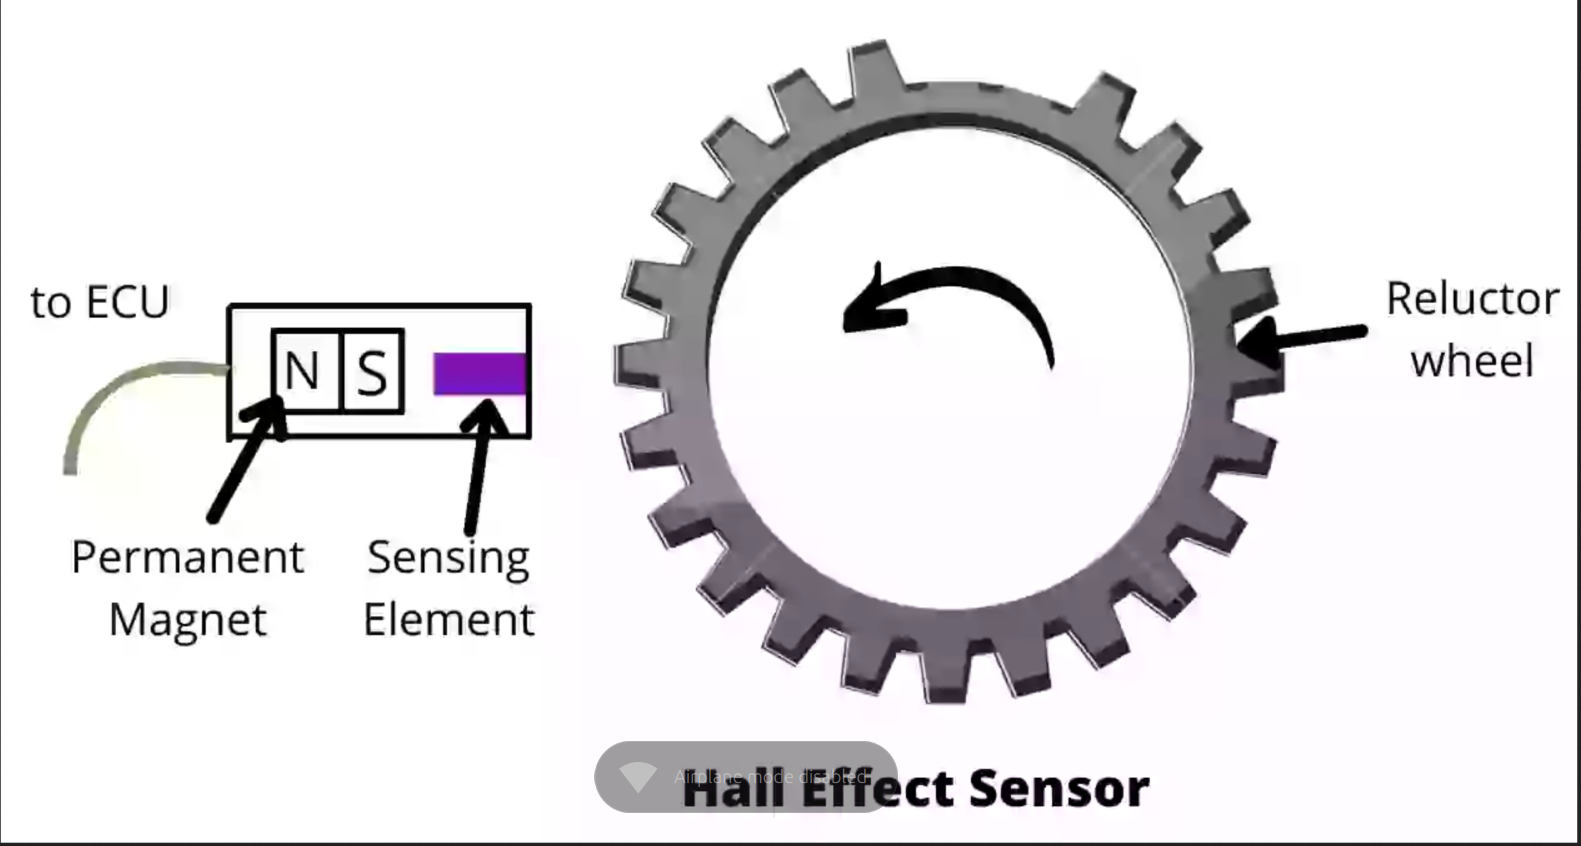
\includegraphics[width=0.45\textwidth]{hall_effect_sensor_rotation}
			\caption{(a) Non contact Ammeter, (b) Rotation sensor}
		\end{figure}
	\end{itemize}
\end{frame}
%
\begin{frame}{Applications of Hall effect}
	\begin{itemize}
		\item Magnetic latch (
\includegraphics[height=2ex]{kiss})	\hfill Proximity sensor
		\item Magnetic switch (
\includegraphics[height=2ex]{slap})	\hfill Rotation sensor
	\end{itemize}
	%
	\begin{figure}
		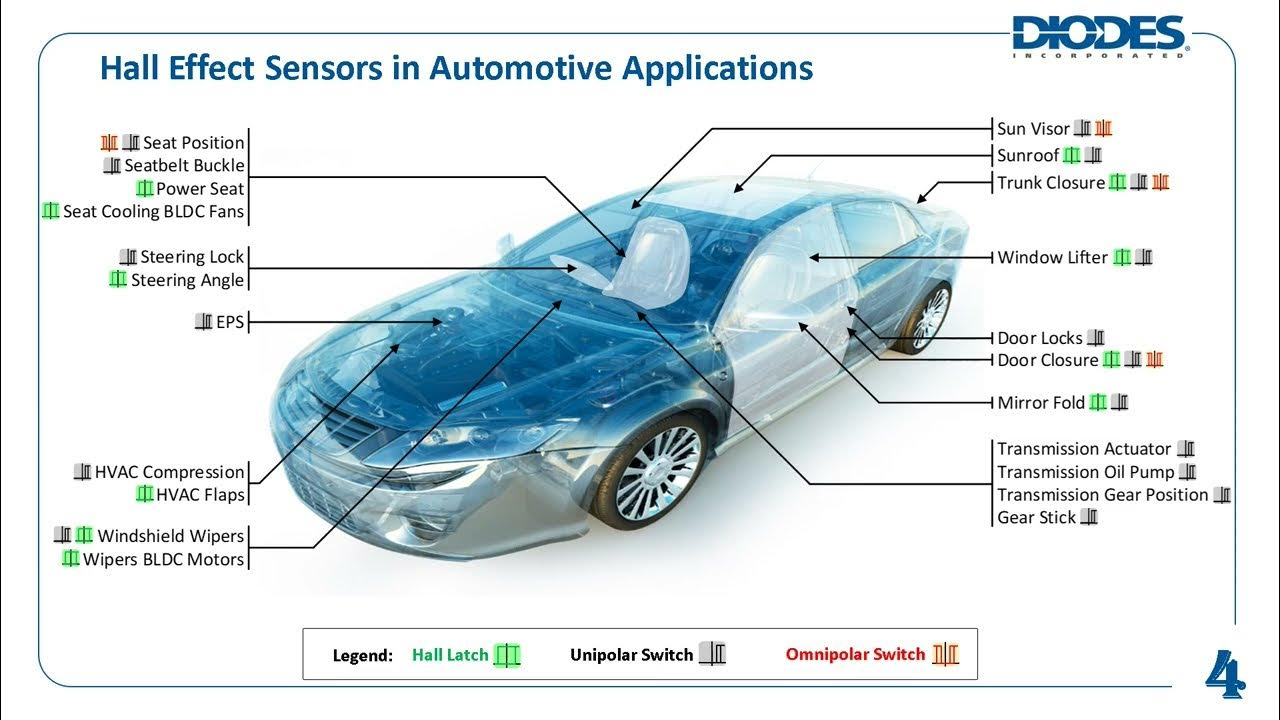
\includegraphics[width=0.9\textwidth]{hall_effect_sensor_car}
		\caption{Reference: \href{https://www.youtube.com/watch?v=tbkrJmo8Fqg}{Youtube link}}
	\end{figure}
\end{frame}
%
\begin{frame}{Summary of Hall effect}
	\begin{itemize}
		\item The Hall effect is a consequence of charged carrier moving in the presence of \textbf{perpendicular} electric and magnetic fields.
		\item The charged carrier is deflected, \textbf{inducing} a Hall voltage.
		\item The polarity of the Hall voltage depends on type of the semiconductor.
		\item The majority carrier concentration and mobility can be determined from the Hall voltage.
	\end{itemize}
\end{frame}
	%\fi
	%
	\section{Concept of Panchabhuta}
	%
	%\ifshowhidden
	%
\againframe{plan}
%
\begin{frame}{Panchabhuta -- Five elements}
	\begin{itemize}
		\item Etymology is Pancha (Sanskrit for five) and bhuta (Sanskrit for elements) 
		\item Fundamental idea in Indian philosophy, Ayurveda, Yoga, and traditional sciences. It explains the composition of the universe, including the human body and mind, in terms of five basic elements.
		\item The Panchabhuta are considered the building blocks of the cosmos. Everything in the universe (macrocosm) and in the human body (microcosm) is made of these five elements in varying proportions.
	\end{itemize}
	%
\end{frame}
%
\begin{frame}{Panchabhuta}
\begin{footnotesize}
		\begin{table}
		\begin{tabular}{l l l l}
			\toprule
			Bhuta	&	Translation 	&	Associated Sense	&	Body part	\\
			\midrule
			Ākāśa & 	Space/Ether		&	Hearing (śabda)	&
			Cavities (Mouth)	\\
			&&& Channels (Nostrils)	\\
			Vāyu	&	Air	&	Touch (sparśa)	&	Spaces (Thorax, Abdomen)	\\
			Agni/Tejas	&	Fire	&	Sight (rūpa)	& digestion, vision \\
			&&& body temperature  \\
			&&& intelligence	\\
			Āpa / Jala	&	Water	&	Taste (rasa)	&	blood, saliva, digestive juices	\\
			&&& plasma, reproductive fluids	\\
			Pṛthvī 	&	Earth	& 	Smell (gandha)	&	bones, teeth, flesh, \\
			&&&	muscles, skin, nails, hair	\\
			\bottomrule
		\end{tabular}
		\caption{{\tiny 1. Ākāśa represents emptiness, vastness, and the medium that allows sound to travel. 2. Vāyu symbolizes movement, motion, and dynamism.
		3. Agni represents transformation, heat, energy, and metabolism.
		4. Jala symbolizes fluidity, cohesion, and life-sustaining properties.
		5. Pṛthvī represents solidity, stability, and structure.}}
	\end{table}
\end{footnotesize}
\end{frame}
%
\begin{frame}{}
	\begin{huge}
		\begin{center}
			End of Unit 1
		\end{center}
	\end{huge}

\end{frame}
	%\fi
	%
\end{document}